\documentclass[12pt,a4paper]{article}
\long\def\/*#1*/{}
\usepackage{verbatim}


\usepackage{listings,chngcntr}
\usepackage{media9}
\usepackage{hyperref}% http://ctan.org/pkg/hyperref
\usepackage{paralist}
\usepackage{xspace}
\usepackage{enumitem}% http://ctan.o\usepackage{amsfonts}rg/pkg/enumitem
\usepackage{amssymb}
\usepackage{amsmath,amsfonts,bm}
\numberwithin{equation}{section}
\DeclareMathOperator{\di}{d\!}
\newcommand*\Eval[3]{\left.#1\right\rvert_{#2}^{#3}}
\usepackage{amsthm}
\newtheorem{theorem}{Theorem}[section]
\newtheorem{corollary}{Corollary}[theorem]
\newtheorem{definition}[theorem]{Definition}
\newtheorem{proposition}[theorem]{Proposition}
\newtheorem{lemma}[theorem]{Lemma}
\usepackage{url}
\usepackage{algorithm}
\usepackage{algpseudocode}
%\usepackage{indentfirst} % paragraph indentation
\usepackage[percent]{overpic}
\makeatletter
\def\BState{\State\hskip-\ALG@thistlm}
\makeatother
\usepackage{mathtools}
%\usepackage{fancyhdr}
%\pagestyle{fancy}
\theoremstyle{definition}
\usepackage{float}
\usepackage[utf8]{inputenc}
\usepackage{cleveref}
\crefname{section}{§}{§§}
\Crefname{section}{§}{§§}
\newcommand{\R}{\mathbb{R}}
 \usepackage{stmaryrd}
 \usepackage{graphicx}
 \usepackage{caption}
 \usepackage{subcaption}
 \usepackage[english]{babel}
\usepackage{color}
\newcommand{\hilight}[1]{\colorbox{yellow}{#1}}
\newcommand{\fakeimage}{{\fboxsep=-\fboxrule\fbox{\rule{0pt}{3cm}\hspace{4cm}}}}
\usepackage{soul}
\usepackage{tikz}
\usetikzlibrary{hobby,shapes,arrows,fit,calc,positioning} 
\newcommand\restr[2]{{% we make the whole thing an ordinary symbol
		\left.\kern-\nulldelimiterspace % automatically resize the bar with \right
		#1 % the function
		\vphantom{\big|} % pretend it's a little taller at normal size
		\right|_{#2} % this is the delimiter
}}
%\newcommand{\innerprod}[2]{\langle\langle #1,#2\rangle\rangle}}
%\newcommand{\energynorm}[2]{\innerprod{\mathcal{A}^{1/2}#1_1}{arg2}}}
\newcommand{\W}{\ensuremath{\Omega}\xspace}
\newcommand{\polygs}[3]{\mathbb{P}^{#1}\qp{#2,#3}}
\newcommand{\Gs}{\mathbb{R}}
\newcommand{\pnorm}[1]{\left|\left|\left|#1\right|\right|\right|}
\newcommand{\norm}[1]{\left|#1\right|}
\newcommand{\Norm}[1]{\left|\left|#1\right|\right|}
\newcommand{\vect}[1]{\textbf{#1}}
\newcommand{\leb}{\text{L}}
\newcommand{\innerprod}[1]{\langle\langle#1\rangle\rangle}
\newcommand{\innerprodsingle}[1]{\langle#1\rangle}
%\newcommand{\innerprod2}[1]{\langle\langle#1\rangle\rangle}
\newcommand{\rP}{\ensuremath{\mathbb P}\xspace}
\newcommand{\poly}[1]{\ensuremath{\rP}^{#1}}
\newcommand{\qp}[1]{\left(#1\right)}
\newcommand{\qpb}[1]{\left(#1\right]}
\newcommand{\qb}[1]{\left[#1\right]}
\newcommand{\rec}[1]{\widehat{{#1}}}
\newcommand{\Normgs}[1]{\left|\left|#1\right|\right|}
\newcommand{\bracegs}[1]{\left\lbrace#1\right\rbrace}
\usepackage{listings}
\usepackage{color}
\usepackage{graphicx, epstopdf}
\usepackage{listings}
\lstset{language=Python}
\renewcommand{\sectionautorefname}{\S}
\setlength{\topmargin}{0.0in}
\setlength{\oddsidemargin}{0.33in}
\setlength{\textheight}{9.0in}
\setlength{\textwidth}{6.0in}
\renewcommand{\baselinestretch}{1.25}
\newtheorem{Defn}[subsection]{Definition}
\newtheorem{Thm}[subsection]{Theorem}
\newtheorem{Proposition}[subsection]{Proposition}
\newtheorem{Lemma}[subsection]{Lemma}
\newtheorem{Rem}[subsection]{Remark}
\newtheorem{Example}[subsection]{Example}
%\linespread{1.3}
\setlist[itemize]{noitemsep, topsep=0pt}
\definecolor{codegreen}{rgb}{0,0.6,0}
\definecolor{codegray}{rgb}{0.5,0.5,0.5}
\lstset{
	frame=single,
	numbers = left,
	basicstyle=\fontsize{9}{11}\ttfamily\linespread{0.85}\ttfamily,
    breaklines=true
}
\setlength{\parindent}{0pt}


\begin{document}
	\begin{titlepage} % Suppresses headers and footers on the title page
		\centering % Centre everything on the title page
		\scshape % Use small caps for all text on the title page
	%	\vspace*{\baselineskip} % White space at the top of the page
		%------------------------------------------------
		%	Title
		%------------------------------------------------
		\rule{\textwidth}{1.6pt}\vspace*{-\baselineskip}\vspace*{2pt} % Thick horizontal rule
		\rule{\textwidth}{0.4pt} % Thin horizontal rule
	%	\vspace{0.75\baselineskip} % Whitespace above the title
		
		{\LARGE Temporal Reconstruction for  \\Second Order Evolution Problems\\} % Title
		
		\vspace{0.75\baselineskip} % Whitespace below the title
		
		\rule{\textwidth}{0.4pt}\vspace*{-\baselineskip}\vspace{3.2pt} % Thin horizontal rule
		\rule{\textwidth}{1.6pt} % Thick horizontal rule
		
		%\vspace{2\baselineskip} % Whitespace after the title block
		
		%------------------------------------------------
		%	Subtitle
		%------------------------------------------------
	%	A Number of Fascinating and Life-changing Templates Presented in a Clear and Concise Way % Subtitle or further description
		
		%\vspace*{1\baselineskip} % Whitespace under the subtitle
		
		%------------------------------------------------
		%	Editor(s)
		%------------------------------------------------
		

		
		\vspace{0.5\baselineskip} % Whitespace before the editors
		
		{\scshape\Large Author:\\ Georgios Sialounas \\$\,$\\ Supervisor: \\Dr Tristan Pryer} % Editor list
		
	%	\vspace{0.5\baselineskip} % Whitespace below the editor list
		
	%	\textit{The University of Reading\\} % Editor affiliation
		
		\vfill % Whitespace between editor names and publisher logo
		
		
		%------------------------------------------------
		%	Publisher
		%------------------------------------------------
		
		\begin{figure}[H]
			\begin{subfigure}[b]{.15\linewidth}
				
\includegraphics[width=\linewidth]{icl_logo_big}
			%	\caption{Velocity in $L^2$: $\left|\left|u-u_h\right|\right|_{L^2}$.}
				\label{icl_logo_big}
			\end{subfigure}
			\begin{subfigure}[b]{.1263\linewidth}
				
\includegraphics[width=\linewidth]{uor_logo_big}
			%	\caption{Velocity in $H^1$: $\left|\left|u-u_h\right|\right|_{H^1}$.}
				\label{uor_logo_big}
			\end{subfigure}
			\centering
		\end{figure}
	\vspace{-14mm}
		\begin{figure}[H]
			
\includegraphics[width=.3\linewidth]{mpe_cdt_logo}
			\centering
		\end{figure}
		\vfill % Whitespace between editor names and publisher logo
		\textit{Report on NSDES\\} % Editor affiliation
		31 August, 2018 % Publication year
		
		%{\large publisher} % Publisher
		
	\end{titlepage}
\pagebreak
\thispagestyle{empty}
\emph{I confirm that this is my work and that it has not been submitted for a degree at another university or institution.\\}
\emph{\\}
\emph{\\}
	\vspace{1\baselineskip} 
\text{Georgios Sialounas}
\pagebreak
\pagebreak
\thispagestyle{empty}
\tableofcontents
\section{Introduction}\label{sec_intro}

In recent years there has been interest in a posteriori error estimation for second order hyperbolic problems (see e.g. \cite{bernardi2005time},\cite{georgoulis2013posteriori},\cite{georgoulis2016posteriori}, \cite{gorynina2018elements},\cite{gorynina2019time},\cite{gorynina2019easily}), albeit belatedly compared to similar advances in parabolic and elliptic problems. The works of \cite{georgoulis2016posteriori}, \cite{gorynina2019time} and  \cite{gorynina2019easily} in particular, are concerned with the temporal aspect of the reconstruction approach.  However, finite difference schemes have not received much attention with regard to a posteriori error estimation, despite the fact that they are frequently in practice,  have not garnered much attention with regard to error estimation.

In this chapter we propose a framework for constructing optimal temporal reconstructions based on the leap-frog scheme for second-order wave-type problems with smooth initial conditions.  The framework we present can be used to facilitate  a posteriori error estimation for finite difference schemes.  We compare a reconstruction obtained from this framework with that of \cite{georgoulis2016posteriori}, on the basis of efficiency.   We also note that the approach we propose can be easily extended to provide residual-type aposteriori estimates for fully discrete finite difference schemes for other evolution problems.  

 

  Although the work in the present chapter uses the same underlying time-marching scheme as \cite{georgoulis2016posteriori}, the reconstruction approach is more similar in spirit to that of  \cite{gorynina2019time} and \cite{gorynina2019easily},  i.e. the fitting of an interpolant in time using the values of the solution at different time-steps.


The rest of the chapter is structured as follows.  In \S \ref{sec:setup} we present the model problem and the leap frog scheme we will use to simulate it.  In \S\ref{sec_reformulation} we present the reformulation of the leap frog scheme, which is what  \cite{georgoulis2016posteriori} used in order to facilitate the derivation of their a posteriori bound.  In \S \ref{sec_bounds} we present the reconstructions we will be comparing and the a-posteriori bound which will be the basis of comparison.   In \S \ref{sec:num_exp} we present the numerical experiments we used to test the reconstructions, followed by the relevant test results.  We conclude the chapter in \S \ref{sec:discussion}, where we  discuss the test results.
\section{Setup}\label{sec:setup}
\subsection{The model problem and notation}\label{subsec_modelprob}
We let $\qp{H,\langle \cdot,\cdot\rangle}$ be a Hilbert space and we let $\mathcal{A}:\qb{0,T}\rightarrow D\qp{\mathcal{A}}$, where $D\qp{\mathcal{A}}$ is the domain of the operator $\mathcal{A}$.  We consider the linear second order hyperbolic problem: find $u:\qb{0,T}\rightarrow \mathbb{R}$ such that
\begin{equation}\label{eq_model_problem}
\begin{aligned}
u''\qp{t}+\mathcal{A}u\qp{t}&=0\quad\text{for}\quad 0\leq t\leq T,\\
u\qp{0}&=u_0,\\
u'\qp{0}&=v_0.
\end{aligned}
\end{equation}

\subsection{Numerical Scheme}\label{subsect_leapfrog}
In this chapter we will consider  the leap-frog scheme for  (\ref{eq_model_problem}).  This is a second-order, explicit scheme for wave-type partial differential equations.  We  subdivide the interval $\qb{0,T}$ into disjoint subintervals $\qpb{t^n, t^{n+1}}$ such that $0=t^0\leq\cdots\leq t^N=T$. The time-step in each subinterval is defined as $\Delta t^n := t^n-t^{n-1},\, n=1,\cdots,N$. 

In order to keep our exposition clear we will work with a constant time-step  $\Delta t^n = \Delta  t = 1/N ,\, \forall n$, although this is not a requirement for the analysis in this section. 
In the exposition that follows we will present a time-discrete version of the Leap-frog scheme instead of a full spatio-temporal discretisation.  This is because we are initially only interested in the temporal aspect of the reconstruction.  

The leapfrog scheme for (\ref{eq_model_problem}) involves finding approximations $U^{n+1}\in D\qp{\mathcal{A}}$ of the exact values $u\qp{t^{n+1}}$ of the solution to (\ref{eq_model_problem}) such that
\begin{equation}\label{eq_model_discrete}
\partial^2U^{n+1}+\mathcal{A}U^n=0,\quad n= 1,\cdots, N-1, 
\end{equation}
where
\begin{equation}
\partial^2U^{n+1}:=\frac{\partial U^{n+1}-\partial U^n}{\Delta t},
\end{equation}
and 
\begin{equation}
\partial U^{n+1}:= \frac{U^{n+1}-U^n}{\Delta t}.
\end{equation}
In order to calculate the quantities in the first time-step, we set $U^0=u_0$ and $\partial U^0:= v_0$ and we calculate $U^1$ using
\begin{equation}
\frac{\partial U^1 - v_0}{\Delta t} + \frac{1}{2}\mathcal{A}U^0 =0.
\end{equation}
\section{Reformulation of the numerical scheme}\label{sec_reformulation}
In \cite{georgoulis2016posteriori}, the  leap-frog scheme, (\ref{eq_model_discrete}), is reformulated as a system of equations two staggered grids.  This system, which is discrete in time, is then recasted in terms of functions which are continuous in time.  The reason for  the reformulation and the subsequent re-casting is to obtain  an a-posteriori bound for the error of (\ref{eq_model_discrete}), which is also the main result from \cite{georgoulis2016posteriori}.  We present a summary of the this process in  \S \ref{subsec_reform_leapfrog}.
\subsection{Reformulated leap frog}\label{subsec_reform_leapfrog}
We introduce the variable
\begin{equation}
V^{n+1/2}:=\partial U^{n+1} \quad\text{for} \quad n=0,\cdots,N-1,
\end{equation}
which will serve as an approximation to $v:=  u'$. We set 
\begin{equation}
V^{-1/2}:=2v_0-V^{1/2}
\end{equation}
and  use this to define
\begin{equation}
U^{-1} := U^0-\Delta t V^{-1/2}.
\end{equation}
Finally, we define
\begin{equation}
\partial V^{n+1/2}:= \frac{V^{n+1/2}-V^{n-1/2}}{\Delta t}, \quad \text{for } \quad n= 0,\cdots, N-1.
\end{equation}
$U^n$ and $V^{n+1/2}$ are used to reformulate (\ref{eq_model_discrete}) the leap-frog scheme as a system of equations on a staggered grid (see Defn. \ref{defn_staggered_midpoint}).
\begin{Defn}[Leap-frog on staggered grids]\label{defn_staggered_midpoint}
	The leap-frog scheme, (\ref{eq_model_discrete}), for (\ref{eq_model_problem}), can be reformulated as a system of equations on a staggered grid as follows
\begin{equation}\label{eq_harmonic_discretization}
\begin{aligned}
\partial U^{n+1} - V^{n+1/2} &= 0,\\
\partial V^{n+1/2} +\mathcal{A}U^n &= 0,\\
U^0 & =0\quad \text{and}\\
V^0 &=1,
\end{aligned}
\end{equation}
for $n= 0,\cdots, N-1$.
\end{Defn}
   We proceed by defining  the piecewise linear interpolator 
\begin{equation}\label{eq_interp_U}
U:\qb{-\Delta t, T}\rightarrow \mathbb{R},
\end{equation}
of the sequence $\bracegs{U^n}_{n=-1}^N$ at $\bracegs{t^n}_{n=-1}^N$, where  $t^n=n\Delta t$ and $t^{-1} = -\Delta t$.  Next, we define the piecewise linear interpolator
\begin{equation}\label{eq_interp_V}
V:\qb{-\Delta t /2, t^{N-1/2}}\rightarrow\mathbb{R},
\end{equation}
 of the sequence $\bracegs{V^{n+1/2}}_{n=-1}^{N-1}$ at $\bracegs{t^{n+1/2}}_{n=-1}^{N-1}$.  
We use (\ref{eq_interp_U}) and (\ref{eq_interp_V}) to define
\begin{equation}
\begin{aligned}
U^{n+1/2}&:=U\qp{t^{n+1/2}}=\frac{1}{2}\qp{U^n+U^{n+1}}\\
V^{n}&:=V\qp{t^{n}}= \frac{1}{2}\qp{V^{n+1/2}+V^{n-1/2}}.
\end{aligned}
\end{equation}
We use  $U^{n+1/2}$ and $V^n$ in conjuction with  (\ref{eq_harmonic_discretization}) to obtain  
\begin{equation}\label{eq_harm_disc_perturbed}
\begin{aligned}
\partial U^{n+1}-\frac{1}{2}\qb{V^{n+1}+V^n}&= -\frac{1}{4}\left(V^{n+3/2}-2V^{n+1/2}+V^{n-1/2}\right) \quad \text{and}\\
\partial V^{n+1/2} +\frac{1}{2}\qp{U^{n+1/2}+U^{n-1/2}}&=\frac{1}{4}\mathcal{A}\left(U^{n+1}-2U^n+U^{n-1}\right)
\end{aligned}
\end{equation}
where the right hand sides are formally defined as the piecewise constant residuals
\begin{equation}
\begin{aligned}
\rho_U&=R_U\left(t\right)|_{\left(t^{n-1/2}, t^{n+1/2}\right]}=\frac{1}{4}\mathcal{A}\left(U^{n+1}-2U^n+U^{n-1}\right)\quad\text{with}\quad \mathcal{A}=I,\\
\rho_V&=R_V\left(t\right)|_{\left(t^n, t^{n+1}\right]}=-\frac{1}{4}\left(V^{n+3/2}-2V^{n+1/2}+V^{n-1/2}\right).
\end{aligned}
\end{equation}
\begin{Rem}[]\label{Rem_opt_perturbation}
Noting that $\rho_u$ and $\rho_V$ are $\mathcal{O}\qp{\Delta t^2}$,  we can view  (\ref{eq_harm_disc_perturbed}) as a second order perturbation of (\ref{eq_harmonic_discretization}).
\end{Rem}
We now introduce two additional interpolants: $U_1$, which is the piecewise linear interpolant of $\bracegs{U^{n+1/2}}_{n=-1}^{N-1}$  at $\bracegs{t^{n+1/2}}_{n=-1}^{N-1}$, and $V_1$, the piecewise linear interpolant of $\bracegs{V^{n}}_{n=0}^{N-1}$ at $\bracegs{t^{n}}_{n=0}^{N-1}$. We use $U_1$ and $V_1$ to re-write (\ref{eq_harm_disc_perturbed}) as
\begin{equation}\label{eq_harm_interpolants}
\begin{aligned}
U'-I_0V_1&=\rho_V,\\
V'+ \mathcal{A}\tilde{I}_0U_1&=\rho_U,
\end{aligned}
\end{equation}
where $\tilde{I}_0$ is the piecewise constant midpoint interpolant on $\qpb{t^{n-1/2}, t^{n+1/2}}$ and ${I}_0$ is the piecewise constant midpoint interpolant on $\qpb{t^{n-1}, t^{n+1}}$. 
\begin{Rem}[Constant residuals $\rho_U$ and $\rho_V$]
As is stated in \cite{georgoulis2016posteriori},  it is not required that the  residuals $\rho_u$ and $\rho_V$ be constant.  However,  constant residuals are sufficient to obtain an optimal a posteriori bound.
\end{Rem}

 
\begin{Rem}\label{Rem_opt_perturbation_cont}
In the same way that (\ref{eq_harm_disc_perturbed}) is a second order perturbation to (\ref{eq_harmonic_discretization}), (\ref{eq_harm_interpolants}) can be viewed as a second order perturbation to
\begin{equation}\label{eq_harmonic_perturbed}
\begin{aligned}
u'- v &= 0,\\
v' +u &= 0.\\
\end{aligned}
\end{equation}
\end{Rem}
In the next section,  (\ref{eq_harm_interpolants}) will serve as the starting point in obtaining the reconstruction of \cite{georgoulis2016posteriori}.
\section{Reconstructions and a-posteriori bounds}\label{sec_bounds}
In this section we explain why we are interested in reconstructions.  We  also define the  reconstructions we will test and  present the relevant a-posteriori bound, which forms the basis for the comparison.  The reader should note that the reconstruction and the results we will present in this section are for the case $\mathcal{A}=I$.  This simplification reduces (\ref{eq_model_problem}) to the simple harmonic oscillator.
\begin{Rem}[Remark on a posteriori estimators]\label{rem_apost_estimator}
 A posteriori error control for a given problem involves establishing an estimate of the form 
\begin{equation}\label{eq_error_estimate}
\Normgs{u-U}\leq \eta\qp{U},
\end{equation}
where $\eta\qp{U}$ is called the\textit{ a-posteriori estimator}.  We would like the estimator to be an explicitly (and preferrably easily) computable quantity.  This implies that $\eta\qp{U}$ should depend on available and explicitly computable quantities, such as the numerical solution  and given problem data. Lastly, we would like $\eta\qp{U}$ to converge with optimal order; that is, with the same order as the error for the chosen numerical scheme.  
\end{Rem}

\begin{Rem}[On reconstructions]
An alternative approach to establishing a posteriori error control for a given problem is for $\eta\qp{\cdot}$ to depend on an intermediate function $\rec{U}$ instead of $U$.   We call $\rec{U}$ the reconstruction of $U$.  Appropriate reconstructions of numerical solutions may have a number of desirable characteristics, which are discussed in detailed in \cite{makridakis2007space}.  In summary:
\begin{itemize}
\item $\rec{U}$ can be a continuous object.  For evolution problems in particular, $U$ may not be continuous in time.  This is the case for various numerical methods, such as for finite difference and finite element methods, where the solution is obtained at discrete points in time.
\item $U-\rec{U}$ should be computable and optimal or bounded by computable and optimal quantities.
\item Let $B\qp{u}$ be the differential operator for the given problem.  Then, $B\qp{\rec{U}}$ should be computable and well-defined.
\item The reconstruction residual $R=B\qp{\rec{U}}$ should be computable or bounded by computable quantities.  Furthermore, it should ideally be an optimal order perturbation of the given problem (see Remarks \ref{Rem_opt_perturbation} and \ref{Rem_opt_perturbation_cont}).
\end{itemize}
\end{Rem}


\begin{Defn}[Reconstruction from \cite{georgoulis2016posteriori}]\label{defn_rec_paper}
The reconstructions for $\rec{U}$ and $\rec{V}$ in \cite[\S3.1]{georgoulis2016posteriori} are given by 
\begin{equation}\label{eq_rec_paper}
\begin{aligned}
\hat{U}&=U^n +\int_{t_n}^{t}\left(V_1+\rho_V\right)\mathrm{d}t, \,\, t\in\qpb{t_n,t_{n+1}}\quad \text{and}\\
\hat{V}&=V^{n-1/2}+\int_{t^{n-1/2}}^{t}\left(-U_1+\rho_U\right)\mathrm{d}t, \,\, t\in\qpb{t_{n-1/2},t_{n+1/2}}.
\end{aligned}
\end{equation}
\end{Defn}
\begin{Rem}
	Note that differentiating (\ref{eq_rec_paper}) in time yields
	\begin{equation}\label{eq_model_recs}
	\begin{aligned}
	\rec{U}'-V_1&=\rho_V \quad\text{and}\\
	\rec{V}'+U_1&=\rho_U.
	\end{aligned}
	\end{equation}
\end{Rem}
We will now present polynomial reconstructions.  Firstly, we will define the space in which they belong. 
\begin{Defn}[Space of piecewise polynomials]\label{defn_space_pwpoly}
	Let $\polygs{q}{\qb{t^{n-1},t^n}}{\mathbb{R}}$ denote the space of real-valued polynomials of degree $q$ in the interval $\qb{t^{n-1}, t^n}$.  Then, we define 
	\begin{equation}
	\mathbb{V}_q:=\bracegs{w:\qb{0,T}\rightarrow\mathbb{R}: w|_{\qb{t^{n-1},t^n}}\in \polygs{q}{\qb{t^{n-1},t^n}}{\mathbb{R}}}
	\end{equation}
	to be the space of piecewise polynomials of degree $q$.
\end{Defn}
\begin{Defn}[Polynomial version of the reconstruction from \cite{georgoulis2016posteriori}]\label{defn_rec_paper_poly}
	The polynomial versions of the reconstructions in Defn. \ref{defn_rec_paper} are given by the functions $\rec{U}\in \mathbb{V}_2$: $\rec{V}\in\mathbb{V}_2$ 
	\begin{equation}\label{eq_rec_paper_poly_alternative}
	\begin{aligned}
	\hat{U}|_{\qb{t^{n} t^{n+1}}}\qp{t}&=c_{0,u}+c_{1,u}\qp{t-t^{n}}+c_{2,u}\qp{t-t^{n}}^2\quad \text{and}\\
	\hat{V}|_{\qb{t^{n-1/2}, t^{n+1/2}}}\qp{t}&=c_{0,v}+c_{1,v}\qp{t-t^{n-1/2}}+c_{2,v}\qp{t-t^{n-1/2}}^2.
	\end{aligned}
	\end{equation}
	The coefficients are obtained using the following conditions:
	\begin{equation}
\begin{aligned}
&\rec{U}|_{\qb{t^n,t^{n+1}}}\qp{t^i}=U^i \quad \text{for}\quad i= n, n+1,\\
&\rec{U}'|_{\qpb{t^n,t^{n+1}}}\qp{t^{n+1}}=-\frac{1}{4}V^{n-1/2}+V^{n+1/2}+\frac{1}{4}V^{n+3/2}\\%-\frac{1}{2}\qp{U^{n+1}+U^n}\\
&\rec{V}|_{\qb{t^{n-1/2},t^{n+1/2}}}\qp{t^i}=V^i \quad \text{for}\quad i= n-1/2, n+1/2,\\
&\rec{V}'|_{\qpb{t^{i-1/2},t^{i+1/2}}}\qp{t^{n+1/2}}=-\frac{1}{4}U^{n+1}-U^n+\frac{1}{4}U^{n-1}
\end{aligned}
	\end{equation}
	or alternatively these conditions
	\begin{equation}\label{eq_alt_conds_paperrec}
	\begin{aligned}
	&\rec{U}|_{\qb{t^n,t^{n+1}}}\qp{t^i}=U^i \quad \text{for}\quad i= n, n+1,\\
	&\rec{U}''|_{\qp{t^n,t^{n+1}}}\qp{t}=\frac{1}{2\Delta t}\qp{V^{n+3/2}-V^{n-1/2}}=-\frac{1}{2}\qp{U^{n+1}+U^n}\\%=-\frac{1}{2}\qp{U^{n+1}+U^n}\\
	&\rec{V}|_{\qb{t^{n-1/2},t^{n+1/2}}}\qp{t^i}=V^i \quad \text{for}\quad i= n-1/2, n+1/2,\\
	&\rec{V}'|_{\qpb{t^{i-1/2},t^{i+1/2}}}\qp{t^{n+1/2}}=-\frac{1}{4}U^{n+1}-U^n+\frac{1}{4}U^{n-1}.
	\end{aligned}
	\end{equation}
	
	Both sets of conditions lead to the coefficients given below
	\begin{equation}\label{eq_coeffs_paperrec}
	\begin{aligned}
	c_{0,u} &= U^{n},\\
	c_{1,u}&=-\frac{1}{4}V^{n+3/2}+V^{n+1/2}+\frac{1}{4}V^{n-1/2},\\
	c_{2,u}&=\frac{1}{4\Delta t}\qp{V^{n+3/2}-V^{n-1/2}}\\%\frac{1}{4\Delta t}\qp{V^{n+3/2}-V^{n-1/2}},\\
	c_{0,v} &= V^{n-1/2},\\
	c_{1,v}&= \frac{1}{4}U^{n+1}-U^n-\frac{1}{4}U^{n-1}\\
	c_{2,v}&=-\frac{1}{4\Delta t}\qp{U^{n+1}-U^{n-1}}=-\frac{1}{4}\qp{V^{n+1/2}+V^{n-1/2}},\\
	\end{aligned}
	\end{equation}
\end{Defn}
\begin{Rem}[Alternative set of conditions for (\ref{eq_rec_paper_poly_alternative})]
The reason for presenting an additional set of conditions, (\ref{eq_alt_conds_paperrec}) for the polynomials (\ref{eq_rec_paper_poly_alternative}), is to facilitate as direct a comparison as possible between this reconstruction and (\ref{eq_rec3_conds}), where $\rec{U}$ is obtained by using a condition on the second derivative.
\end{Rem}


\begin{Defn}[ ]\label{defn_our_rec3}
	The reconstruction, $\qp{\rec{U},\rec{V}}$ of the numerical solution $\qp{U,V}$ of (\ref{eq_harmonic_discretization}) on a staggered grid consists of the unique functions $\rec{U}\in \mathbb{V}_2$, $\rec{V}\in\mathbb{V}_3$ satisfying
	\begin{equation}\label{eq_rec3_conds}
	\begin{aligned}
	&\rec{U}\qp{t^i}=U^i \quad \text{for}\quad i= n, n+1,\\
	&\rec{U}''|_{\qp{t^n,t^{n+1}}}\qp{t}=-U^n,\quad\forall t\in\qp{t^n, t^{n+1}}\\
	&\rec{V}\qp{t^i}=V^i \quad \text{for}\quad i= n-1/2, n+1/2,\\
	&\rec{V}'\qp{t^i}=-\rec{U}\qp{t^i},\quad i = n-1/2, \, n+1/2\\
	\end{aligned}
	\end{equation}
	This set of conditions leads to the coefficients given below
	\begin{equation}\label{eq_coeffs_ours}
	\begin{aligned}
	c_{0,u} &= U^{n},\\
	c_{1,u}&=\frac{1}{\Delta t}\qp{U^{n+1}-U^n+\frac{1}{2}\Delta t^2 U^n}\\
	c_{2,u}&=-\frac{U^n}{2}\\%\frac{1}{4\Delta t}\qp{V^{n+3/2}-V^{n-1/2}},\\
	c_{0,v} &= V^{n-1/2},\\
	c_{1,v}&=-\rec{U}\qp{t^{n-1/2}}\\
	c_{2,v}&=\frac{1}{\Delta t}\qp{\rec{U}\qp{t^{n+1/2}}-\rec{U}\qp{t^{n-1/2}}}+\frac{3}{\Delta t^2}\qp{V^{n+1/2}-V^{n-1/2}+\Delta t \rec{U}\qp{t^{n-1/2}}}\\
	c_{3,v}&=-\frac{1}{\Delta t^2}\qp{\rec{U}\qp{t^{n+1/2}}-\rec{U}\qp{t^{n-1/2}}}-\frac{2}{\Delta t^3}\qp{V^{n+1/2}-V^{n-1/2}+\Delta t \rec{U}\qp{t^{n-1/2}}} 
	\end{aligned}
	\end{equation}
\end{Defn}

 \/*
\begin{Defn}[ ]\label{defn_our_rec}
	The reconstruction, $\qp{\rec{U},\rec{V}}$ of the numerical solution $\qp{U,V}$ of (\ref{eq_harmonic_discretization}) consists of the unique functions $\rec{U}\in \mathbb{V}_2$, $\rec{V}\in\mathbb{V}_2$ satisfying
	\begin{equation}
	\begin{aligned}
	&\rec{U}|_{\qb{t^n,t^{n+1}}}\qp{t^i}=U^i \quad \text{for}\quad i= n, n+1,\\
	&\rec{U}''|_{\qb{t^n,t^{n+1}}}\qp{t^n}=-U^n,\\
	&	\rec{V}|_{\qb{t^n,t^{n+1}}}\qp{t^{i}}=V^{i}\quad \text{for}\quad i= n, n+1\quad\text{and}\\
	&	\rec{V}'|_{\qb{t^n,t^{n+1}}}\qp{t^n}=-U^n.\\
	\end{aligned}
	\end{equation}
\end{Defn}
\begin{Defn}[ ]\label{defn_our_rec2}
	The reconstruction, $\qp{\rec{U},\rec{V}}$ of the numerical solution $\qp{U,V}$ of (\ref{eq_harmonic_discretization}) consists of the unique functions $\rec{U}\in \mathbb{V}_2$, $\rec{V}\in\mathbb{V}_3$ satisfying
	\begin{equation}\label{eq_rec2_conds}
	\begin{aligned}
	&\rec{U}|_{\qb{t^n,t^{n+1}}}\qp{t^i}=U^i \quad \text{for}\quad i= n, n+1,\\
	&\rec{U}''|_{\qb{t^n,t^{n+1}}}\qp{t^n}=-U^n,\\
     &\rec{V}|_{\qb{t^n,t^{n+1}}}\qp{t^i}=V^i \quad \text{for}\quad i= n, n+1,\\
      &\rec{V}'|_{\qb{t^n,t^{n+1}}}\qp{t^n}=-\rec{U}|_{\qb{t^n,t^{n+1}}}\qp{t^n}\\
            &\rec{V}''|_{\qb{t^n,t^{n+1}}}\qp{t^n}=-\rec{U}'|_{\qb{t^n,t^{n+1}}}\qp{t^n}\\
	\end{aligned}
	\end{equation}
\end{Defn}

\begin{Rem}[Conditions for $\hat{\textbf{V}}$ from Defn. \ref{defn_our_rec2}]
	The nodal equivalence conditions for $\rec{V}$ in (\ref{eq_rec2_conds}) fixes two of the four coefficients required to define a third order polynomial in the interval $\qb{t^{n-1}, t^n}$.  The remaining two coefficients will be obtained by the relation we want between $\rec{V}$ and $\rec{U}$, as shown in Example \ref{example:sample_rec}.  
\end{Rem}
\begin{Example}[Example of a recosntruction based on Defn. \ref{defn_our_rec2}]\label{example:sample_rec}
The reconstructions $\rec{U}$  and for $\rec{V}$ are constructed as follows.
\begin{equation}
\begin{aligned}
\text{Let}\quad\hat{U}\qp{t}|_{\qb{{t_n, t_{n+1}}}}&= c_{0,u} +c_{1,u}\qp{t-t_n} +c_{2,u}\qp{t-t_n}^2,\quad\text{where}\\
c_{0,u} &= U^n,\\
c_{1,u} &= \frac{1}{\Delta t}\qb{U^{n+1}-U^n + \frac{\Delta t^2}{2}U^n},\quad\text{and}\\
c_{2,u} &= -U^n/2\quad \text{and}\\
\hat{V}\qp{t}|_{\qb{{t_n, t_{n+1}}}}&= c_{0,v} +c_{1,v}\qp{t-t_n} +c_{2,v}\qp{t-t_n}^2+c_{3,v}\qp{t-t_n}^3,\quad\text{where}\\
c_{0,v} &=\frac{1}{2}\qp{V^{n-1/2}+V^{n+1/2} },\\
c_{1,v} &= -c_{0,u},\\
c_{2,v} &= -\frac{1}{2}c_{1,u}\text{  and}\\
c_{3,v} &= \frac{1}{2}\qp{V^{n+1/2}+V^{n+3/2} }-c_{0,v}- c_{1,v}\Delta t- c_{2,v}\Delta t^2
\end{aligned}
\end{equation}
\end{Example}



\begin{Rem}[Conditions for $\hat{\textbf{V}}$ from Defn. \ref{defn_our_rec2}]
Two of the coefficients for $\rec{V}$ in Defn. \ref{defn_our_rec2} come from nodal equivalence.  We define the remaining two coefficients  by imposing, in an approximate sense, the relation between $\rec{V}$ and $\rec{U}'$ that is indicated by the second equation in (\ref{eq_harmonic_perturbed}).  This is an effort to make the bound sharper. The reason we stop here rather than opting for a minimization approach is to keep the framework as general as possible rather than optimizing it for a specific problem.
\end{Rem}
*/
\subsection{Error equation and estimators}\label{subsec_error_estimators}
\begin{Defn}[Errors]\label{defn:errors}
We define the following error equations for $u$ and $v$ as
\begin{equation}\label{eq_err_rec_uv}
\begin{aligned}
\hat{e}_U&:=u-\hat{U} \quad \text{and}\\
\hat{e}_V&:=v-\hat{V}.
\end{aligned}
\end{equation}
\end{Defn}

\begin{Defn}[Error equations]
The error equations (see \cite[eq. 3.2]{georgoulis2016posteriori}) are given by 
\begin{equation}\label{eq_error_eqs}
\begin{aligned}
\hat{e}'_V+\mathcal{A}\hat{e}_U&=\mathcal{R}_1\\
\hat{e}'_U-\hat{e}_V&=\mathcal{R}_2,
\end{aligned}
\end{equation}
where  $\mathcal{R}_{1,2}$ are residuals which depend upon the chosen reconstruction.
\end{Defn}
\begin{Rem}[Form of the error equations]
Notice that the PDE system satisfied by the error equations (\ref{eq_err_rec_uv}) is the same as as the underlying PDE system (\ref{eq_harmonic_perturbed}) with an additional forcing term depending on the reconstruction residual.  The significance of this is that the analysis required to obtain an a-posteriori error-bound can be carried out using the stability framework of the underlying PDE.
\end{Rem}
%We will use the following errors to assess the behaviour of the estimators:
%\begin{equation}\label{eq_error_definitions}
%e_R:= \qp{\hat{e}_U, \hat{e}_V},\quad e_L:= e_R +\qp{U-\hat{U}, V-\hat{V}}= \qp{u-U, v-V}.
%\end{equation}
\/*
 In the case of the reconstruction of \cite{georgoulis2016posteriori}, in light of (\ref{eq_model_recs}) , these residuals are given by
\begin{equation}\label{eq_residuals_paper}
\begin{aligned}
\mathcal{R}_1&:=-\left(\hat{U}-U_1\right)-\rho_U\\
\mathcal{R}_2&:=\hat{V}-V_1-\rho_V,
\end{aligned}
\end{equation}
*/
The forms of $\mathcal{R}_1$ and $\mathcal{R}_2$ are obtained by substituting the reconstructions $\rec{U}$ and $\rec{V}$ for $u$ and $v$ respectively in (\ref{eq_harmonic_perturbed}):
\begin{equation}\label{eq_residuals_our}
\begin{aligned}
\mathcal{R}_1&:=\hat{V}'+\hat{U}\\
\mathcal{R}_2&:=\hat{U}'-\hat{V}.
\end{aligned}
\end{equation}
$\mathcal{R}_1$ and $\mathcal{R}_2$ are used in the computation of the bound in \cite[Thm 3.1]{georgoulis2016posteriori}, which we present in Thm. \ref{thm:bound}.
\begin{Rem}[Set of residuals used in testing]
Note that the set of residuals $\mathcal{R}_1$ and $\mathcal{R}_2$ we present in (\ref{eq_residuals_our}) is not the same as the one used in \cite{georgoulis2016posteriori}.  However, in order to establish a clear comparison for the performance of the reconstructions, we will be using the residulas given by (\ref{eq_residuals_our}) for both of the reconstructions we will test.  The reader should note that it has been confirmed by testing that the behaviour of the bound we will test in the following sections is the same for (\ref{eq_residuals_our}) as it is for the original residuals from \cite{georgoulis2016posteriori}.  The relevant results have been omitted for the sake of clarity of exposition.
\end{Rem}



Let $\Phi=\qp{\phi_1, \phi_2}$, $\Psi =\qp{\psi_1,\psi_2}\in D\qp{\mathcal{A}}\times H$ where $D\qp{\mathcal{A}}$ and $H$ are defined in \S \ref{sec:setup}.  The inner product used in the computation is the standard energy inner product on $\qb{D\qp{\mathcal{A}}\times H}^2$
\begin{equation}\label{defn_innerprod}
\langle\langle \Phi,\Psi \rangle\rangle:= \langle \mathcal{A}^{1/2}\phi_1, \mathcal{A}^{1/2}\psi_1  \rangle + \langle \phi_1. \psi_1  \rangle,
\end{equation}
which induces the norm
\begin{equation}
\pnorm{\Phi} = \qp{\Normgs{\mathcal{A}^{1/2}\phi_1} + \Normgs{\phi_2}}^{1/2}.
\end{equation}
In the case we are interested in, where $\mathcal{A}=I$,  this simplifies to
\begin{equation}
\left|\left|\left|\left(\mathcal{R}_2, \mathcal{R}_1\right)\right|\right|\right| = (\mathcal{R}_2^2 +\mathcal{R}_1^2)^{1/2}.
\end{equation}
This leads us to the main result from \cite[Thm 3.1]{georgoulis2016posteriori}.  Before we present the result and its proof we include a helpful Lemma.
\begin{Lemma}[Cauchy Inequality with $\epsilon$]
	Let $a,b \in \mathbb{R}$ and $\epsilon>0]$.  Then
	\begin{equation}\label{eq_cauchy_ineq_eps}
	ab\leq \epsilon a^2 +\frac{1}{4\epsilon}b^2.
	\end{equation}
\end{Lemma}
\begin{proof}
	\begin{equation*}
	0\leq \qp{\sqrt{\epsilon}a-\frac{1}{2\sqrt{\epsilon}b}}^2\implies ab\leq \epsilon a^2 +\frac{1}{4\epsilon}b^2
	\end{equation*}
\end{proof}
\begin{Thm}[A-posteriori error bound for (\ref{eq_model_problem})]\label{thm:bound}
Let $u$ be the solution of (\ref{eq_model_problem}), $\hat{e}_u:=u-\rec{U}$ and $\hat{e}_v:=v-\rec{V}$ .  Then the following a posteriori error estimate holds
\begin{equation}\label{eq_bound}
\sup_{t\in\qb{0,t^N}}\pnorm{\qp{\hat{e}_U,\hat{e}_V}\qp{t}}^2\leq
2\pnorm{\qp{\hat{e}_U,\hat{e}_V}\qp{0}}^2+
4\qp{\int_0^{t^N}\pnorm{\qp{\mathcal{R}_2,\mathcal{R}_1}}\mathrm{d}t}^2,
\end{equation}
where $\mathcal{R}_1$ and $\mathcal{R}_2$ are defined in (\ref{eq_residuals_our}).
\end{Thm}
\begin{proof}
The estimate follows by applying energy arguments to (\ref{eq_error_eqs}).  The starting point is to test $\qp{\hat{e}_U', \hat{e}_V'}$ with $\qp{\hat{e}_U, \hat{e}_V}$, giving
\begin{equation}
\begin{aligned}
\frac{1}{2}\frac{\mathrm{d}}{\mathrm{d}t}\pnorm{\qp{\hat{e}_U,\hat{e}_V}}^2
    &=\innerprod{\qp{\hat{e}_U', \hat{e}_V'}, \qp{\hat{e}_U, \hat{e}_V}}.
\end{aligned}
\end{equation}
We now use (\ref{defn_innerprod}) to obtain 
\begin{equation}
\begin{aligned}
\innerprod{\qp{\hat{e}_U', \hat{e}_V'}, \qp{\hat{e}_U, \hat{e}_V}}
&=\innerprodsingle{\mathcal{A}\hat{e}_U',\hat{e}_U}+\innerprodsingle{\hat{e}_V',\hat{e}_V}\\
&=\innerprodsingle{\mathcal{A}\hat{e}_V,\hat{e}_U}
+\innerprodsingle{\mathcal{A}\mathcal{R}_2,\hat{e}_U}
-\innerprodsingle{\mathcal{A}\hat{e}_U,\hat{e}_V}
+\innerprodsingle{\mathcal{R}_1,\hat{e}_V}.
\end{aligned}
\end{equation}
Substituting in from (\ref{eq_error_eqs}) gives 
\begin{equation}
\begin{aligned}
\innerprodsingle{\mathcal{A}\hat{e}_U',\hat{e}_U}+\innerprodsingle{\hat{e}_V',\hat{e}_V}&
=\innerprodsingle{\mathcal{A}\hat{e}_V,\hat{e}_U}
+\innerprodsingle{\mathcal{A}\mathcal{R}_2,\hat{e}_U}
-\innerprodsingle{\mathcal{A}\hat{e}_U,\hat{e}_V}
+\innerprodsingle{\mathcal{R}_1,\hat{e}_V}.
\end{aligned}
\end{equation}
We then use the Cauchy-Schwarz inequality to obtain
\begin{equation}\label{eq_bound_cauchyschwarz}
\frac{1}{2}\frac{\mathrm{d}}{\mathrm{d}t}\pnorm{\qp{\hat{e}_U,\hat{e}_V}}^2
  \leq  \pnorm{\qp{\mathcal{R}_2,\mathcal{R}_1}} \pnorm{\qp{\hat{e}_U,\hat{e}_V}}
\end{equation}
In what follows, we will be using the $\leb^\infty$ norm in time
\begin{equation}\label{eq_sup_pnorm}
\pnorm{\qp{\hat{e}_U, \hat{e}_V}\qp{\tau}}=\sup_{t\in\qb{0,t^N}}\pnorm{\qp{\hat{e}_U, \hat{e}_V}\qp{t}}.
\end{equation}
Integrating (\ref{eq_bound_cauchyschwarz}) from $0$ to $\tau$, where $\tau$ is defined in (\ref{eq_sup_pnorm}), yields
\begin{equation}
\small
\begin{aligned}
\frac{1}{2}\pnorm{\qp{\hat{e}_U, \hat{e}_V}\qp{\tau}}^2&\leq
\frac{1}{2}\pnorm{\qp{\hat{e}_U, \hat{e}_V}\qp{0}}^2
+\int_0^\tau\pnorm{\qp{\mathcal{R}_2,\mathcal{R}_1}\qp{t}} \pnorm{\qp{\hat{e}_U,\hat{e}_V}\qp{t}}\mathrm{d}t\\
&\leq \frac{1}{2}\pnorm{\qp{\hat{e}_U, \hat{e}_V}\qp{0}}^2
+\pnorm{\qp{\hat{e}_U,\hat{e}_V}\qp{\tau}}\int_0^\tau\pnorm{\qp{\mathcal{R}_2,\mathcal{R}_1}\qp{t}} \mathrm{d}t,
\end{aligned}
\end{equation}
where we have used (\ref{eq_sup_pnorm}).
Using (\ref{eq_cauchy_ineq_eps}) with $\epsilon=1$, $a=\int_0^\tau\pnorm{\qp{\mathcal{R}_2,\mathcal{R}_1}\qp{t}} \mathrm{d}t$ and $b=\pnorm{\qp{\hat{e}_U,\hat{e}_V}\qp{\tau}}$ for the product term on the rhs and multiplying by two throughout yields the required result.
\end{proof}

\begin{Rem}[The error at $t=0$]
	Notice the constant $2\pnorm{\qp{\hat{e}_U,\hat{e}_V}\qp{0}}^2$ in (\ref{eq_bound}).  The significance of this is that the initial error, depending on the chosen reconstruction, may not be $0$.  This is because of the use of a staggered grid.
\end{Rem}

\/*

Before we proceed we will prove an additional bound.  In order to do this we will use an addional result
\begin{Proposition}\label{lemma:L2_simplification}[$\leb_2$ simplification rule] If $\vect{a},\, \vect{b}\in \mathbb{R}^N,\, N\in \mathbb{N}$, $c\in \mathbb{R}$ and $f\,g \in \leb_2\qp{D}$ for some measurable domain $D$ are such that 
	\begin{equation*}
\norm{\vect{a}}^2 +\Norm{{f}}^2\leq c^2+\vect{a}^T\vect{b}+\int_D fg,
 	\end{equation*}
then
\begin{equation}
\qp{\norm{\vect{a}}^2 +\Norm{{f}}^2}^{1/2}\leq \norm{c}+\qp{\norm{{b}}^2+\Norm{g}^2}^{1/2}
\end{equation}
\end{Proposition}

\begin{Lemma}[Second a-posteriori error bound for (\ref{eq_model_problem})]
	Let $u$ be the solution of (\ref{eq_model_problem}), $\hat{e}_u:=u-\rec{U}$ and $\hat{e}_v:=v-\rec{V}$ .  Then the following error estimate holds
	\begin{equation}\label{eq_bound_2}
	\sup_{t\in\qb{0,t^N}}\pnorm{\qp{\hat{e}_U,\hat{e}_V}\qp{t}}\leq
	\pnorm{\qp{\hat{e}_U,\hat{e}_V}\qp{0}}+
	2{\int_0^{t^N}\pnorm{\qp{\mathcal{R}_2,\mathcal{R}_1}}\mathrm{d}t},
	\end{equation}
	where $\mathcal{R}_1$ and $\mathcal{R}_2$ are defined in (\ref{eq_residuals_our}).
\end{Lemma}
\begin{proof}
We use  Lemma  \ref{lemma:L2_simplification} with $\vect{a}=\frac{1}{\sqrt{2}}\pnorm{\qp{\hat{e}_U, \hat{e}_V}\qp{\tau}}$, $\vect{b}=\sqrt{2}\int_0^\tau\pnorm{\qp{\mathcal{R}_2,\mathcal{R}_1}\qp{t}} \mathrm{d}t$ and $c = \frac{1}{\sqrt{2}}\pnorm{\qp{\hat{e}_U, \hat{e}_V}\qp{0}}$ and we obtain the required result.
\end{proof}

*/

\section{Numerical Experiments}\label{sec_num_exp}
The objectives in this section are to study the performance of the indicator 
\begin{equation}\label{eq_bound_test}
\eta_1=\qp{2\pnorm{\qp{\hat{e}_U,\hat{e}_V}\qp{0}}^2+
	4\qp{\int_0^{t^N}\pnorm{\qp{\mathcal{R}_2,\mathcal{R}_1}}\mathrm{d}t}^2}^{1/2}
\end{equation}
for the reconstructions in Defns. (\ref{defn_rec_paper}) and (\ref{defn_our_rec3})  and to compare their performance on the basis of optimality and efficiency.  In this case, an efficient indicator whose effectivity index is one that is closer to one (see (\ref{eq_EI})). To this extend we introduce the error
\begin{equation}\label{eq_error_eR}
e_R :=\qp{\hat{e}_U,\hat{e_V}},
\end{equation}
where $\hat{e_U}$ and $\hat{e}_V$ are defined in (\ref{eq_err_rec_uv}).  
The comparison will be on the basis of the Effectivity Index (EI) of the error indicators and of the Estimated Order of Convergence (EOC).
\begin{Defn}[Effectivity Index (EI)] The effectivity index of an error indicator $\eta_1$ compared to a given error at time $t$ is defined as
\begin{equation}\label{eq_EI}
EI\qp{error\qp{t}, \eta_1\qp{t}} := \frac{\eta_1\qp{t}}{error\qp{t}}
\end{equation}
\end{Defn}

\begin{Defn}[Estimated Order of Convergence (EOC)] Given two sequences $a\qp{i}$ and $h\qp{i}\downarrow 0$, we define the estimated order of convergence as
\begin{equation}
EOC\qp{a,h;i} = \frac{log\qp{a\qp{i+1}/a\qp{i}}}{log\qp{h\qp{i+1}/h\qp{i}}}.
\end{equation}
\end{Defn}

\subsection{Discrete Formulation}\label{subsec_disc_form}
We discretize (\ref{eq_harmonic_perturbed}) using
\begin{equation}
\begin{aligned}
\partial U^{n+1} - V^{n+1/2} &= 0\\
\partial V^{n+1/2} +U^n &= 0\\
U^0 & =u_0\\
V^0 &=v_0.
\end{aligned}
\quad \text{for } \quad n= 0,\cdots, N-1,
\end{equation}
for several different pairs of initial conditions $\qp{u_0, v_0}$.  In each case we will obtain  $U^1$ and $V^{1/2}$ using
\begin{equation}
\begin{aligned}
U^1&=U^0+\Delta t V^0 -\frac{\Delta t^2}{2}U^0\quad\text{and}\\
V^{1/2} &= \frac{1}{\Delta t}\qp{U^1-U^0}.
\end{aligned}
\end{equation}


\/*
\subsubsection{$u_0=0,\, v_0=1$}
\begin{figure}[H]
	\hspace{-3cm}
	%\centering
	\includegraphics[scale=0.55]{fig_LeapFrogplots_1x5_sin_IC_harmonic_order_2_u0_v1_rec1}	
	\caption{Reconstruction from Defn. \ref{defn_our_rec}. (from left to right) Error $e_R$ given by (\ref{eq_error_eR}), Estimator $\eta_1$ given by \ref{eq_bound_test}, Error $e_L$ given by  (\ref{eq_error_eL}). EOC error, EOC Estimator, Effectivity Index.}
	\label{fig_all_in_one_our_rec_1_u0_v1}
\end{figure}

\begin{figure}[H]
	\hspace{-3cm}
	%\centering
	\includegraphics[scale=0.55]{fig_LeapFrogplots_1x5_sin_IC_harmonic_order_2_u0_v1_rec2}	
	\caption{Reconstruction from Defn. \ref{defn_our_rec2}. (from left to right) Error $e_R$ given by (\ref{eq_error_eR}), Estimator $\eta_1$ given by \ref{eq_bound_test}, Error $e_L$ given by  (\ref{eq_error_eL}). EOC error, EOC Estimator, Effectivity Index.}
	\label{fig_all_in_one_our_rec_2_u0_v1}
\end{figure}

\begin{figure}[H]
	\hspace{-3cm}
	%\centering
	\includegraphics[scale=0.55]{fig_LeapFrogplots_1x5_sin_IC_harmonic_paperrec_u0_v1}	
	\caption{Paper rec.  (from left to right) Error $e_R$ given by (\ref{eq_error_eR}), Estimator $\eta_1$ given by \ref{eq_bound_test}, Error $e_L$ given by  (\ref{eq_error_eL}). EOC error, EOC Estimator, Effectivity Index.}
	\label{fig_all_in_one_paper_rec_2_u0_v1}
\end{figure}

\subsubsection{$u_0=1,\, v_0=0$}
\begin{figure}[H]
	\hspace{-3cm}
	%\centering
	\includegraphics[scale=0.55]{fig_LeapFrogplots_1x5_sin_IC_harmonic_order_2_u1_v0_rec1}	
	\caption{Reconstruction from Defn. \ref{defn_our_rec}. (from left to right) Error $e_R$ given by (\ref{eq_error_eR}), Estimator $\eta_1$ given by \ref{eq_bound_test}, Error $e_L$ given by  (\ref{eq_error_eL}). EOC error, EOC Estimator, Effectivity Index.}
	\label{fig_all_in_one_our_rec_1_u1_v0}
\end{figure}

\begin{figure}[H]
	\hspace{-3cm}
	%\centering
	\includegraphics[scale=0.55]{fig_LeapFrogplots_1x5_sin_IC_harmonic_order_2_u1_v0_rec2}	
	\caption{Reconstruction from Defn. \ref{defn_our_rec2}. (from left to right) Error $e_R$ given by (\ref{eq_error_eR}), Estimator $\eta_1$ given by \ref{eq_bound_test}, Error $e_L$ given by  (\ref{eq_error_eL}). EOC error, EOC Estimator, Effectivity Index.}
	\label{fig_all_in_one_our_rec_2_u1_v0}
\end{figure}

\begin{figure}[H]
	\hspace{-3cm}
	%\centering
	\includegraphics[scale=0.55]{fig_LeapFrogplots_1x5_sin_IC_harmonic_paperrec_u1_v0}	
	\caption{Paper rec.  (from left to right) Error $e_R$ given by (\ref{eq_error_eR}), Estimator $\eta_1$ given by \ref{eq_bound_test}, Error $e_L$ given by  (\ref{eq_error_eL}). EOC error, EOC Estimator, Effectivity Index.}
	\label{fig_all_in_one_paper_rec_2_u1_v0}
\end{figure}


\subsubsection{$u_0=1,\, v_0=1$}

\begin{figure}[H]
	\hspace{-3cm}
	%\centering
	\includegraphics[scale=0.55]{fig_LeapFrogplots_1x5_sin_IC_harmonic_order_2_u1_v1_rec1}	
	\caption{Reconstruction from Defn. \ref{defn_our_rec}. (from left to right) Error $e_R$ given by (\ref{eq_error_eR}), Estimator $\eta_1$ given by \ref{eq_bound_test}, Error $e_L$ given by  (\ref{eq_error_eL}). EOC error, EOC Estimator, Effectivity Index.}
	\label{fig_all_in_one_our_rec_1_u1_v1}
\end{figure}

\begin{figure}[H]
	\hspace{-3cm}
	%\centering
	\includegraphics[scale=0.55]{fig_LeapFrogplots_1x5_sin_IC_harmonic_order_2_u1_v1_rec2}	
	\caption{Reconstruction from Defn. \ref{defn_our_rec2}. (from left to right) Error $e_R$ given by (\ref{eq_error_eR}), Estimator $\eta_1$ given by \ref{eq_bound_test}, Error $e_L$ given by  (\ref{eq_error_eL}). EOC error, EOC Estimator, Effectivity Index.}
	\label{fig_all_in_one_our_rec_2_u1_v1}
\end{figure}

\begin{figure}[H]
	\hspace{-3cm}
	%\centering
	\includegraphics[scale=0.55]{fig_LeapFrogplots_1x5_sin_IC_harmonic_paperrec_u1_v1}	
	\caption{Paper rec.   (from left to right) Error $e_R$ given by (\ref{eq_error_eR}), Estimator $\eta_1$ given by \ref{eq_bound_test}, Error $e_L$ given by  (\ref{eq_error_eL}). EOC error, EOC Estimator, Effectivity Index. }
	\label{fig_all_in_one_paper_rec_2_u1_v1}
\end{figure}


*/
\subsection{Test results}\label{sec:num_exp}
\subsection*{$u_0=0, v_0= 1$}
\/*
\begin{figure}[H]
	\hspace{-3cm}
	%\centering
	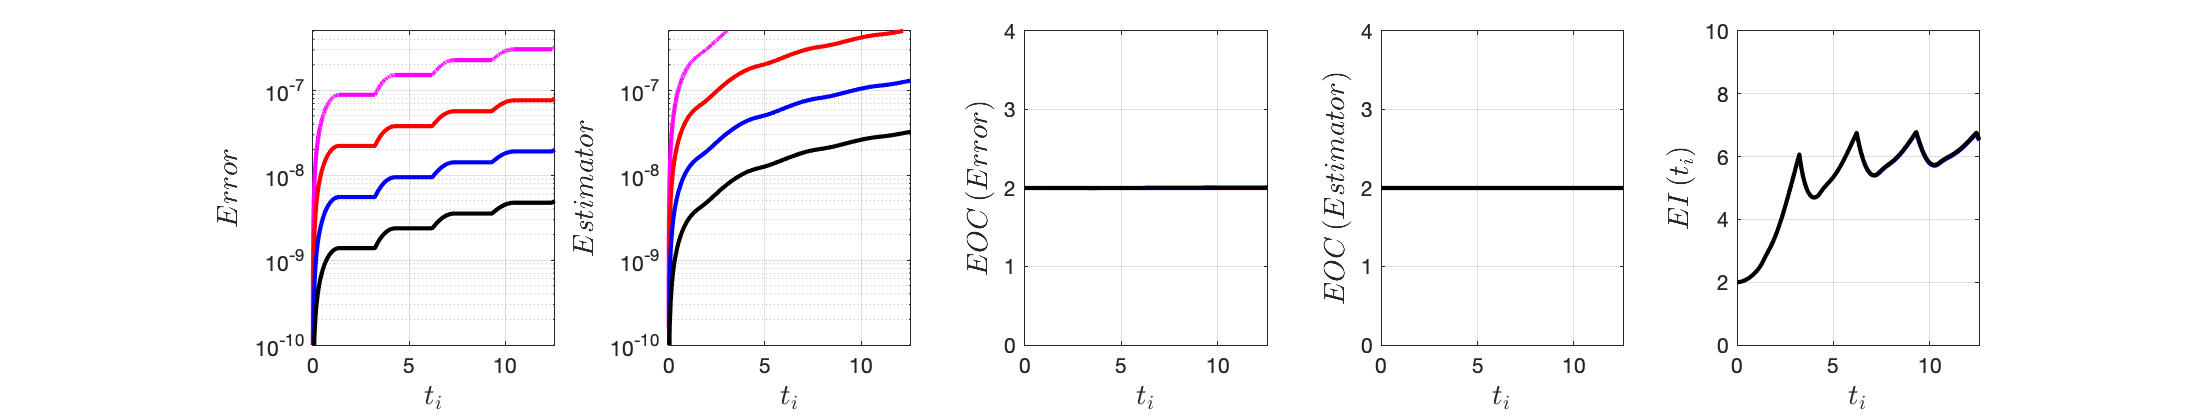
\includegraphics[scale=0.55]{fig_LeapFrogplots_1x5_sin_IC_harmonic_order_2_u0_v10_rec_george}	
	\caption{Reconstruction from Defn. \ref{defn_our_rec}. (from left to right) Error $e_R$ given by (\ref{eq_error_eR}), Estimator $\eta_1$ given by \ref{eq_bound_test}, EOC error, EOC Estimator, Effectivity Index.}
	\label{fig_all_in_one_our_rec_george_u0_v10}
\end{figure}

\begin{figure}[H]
	\hspace{-3cm}
	%\centering
	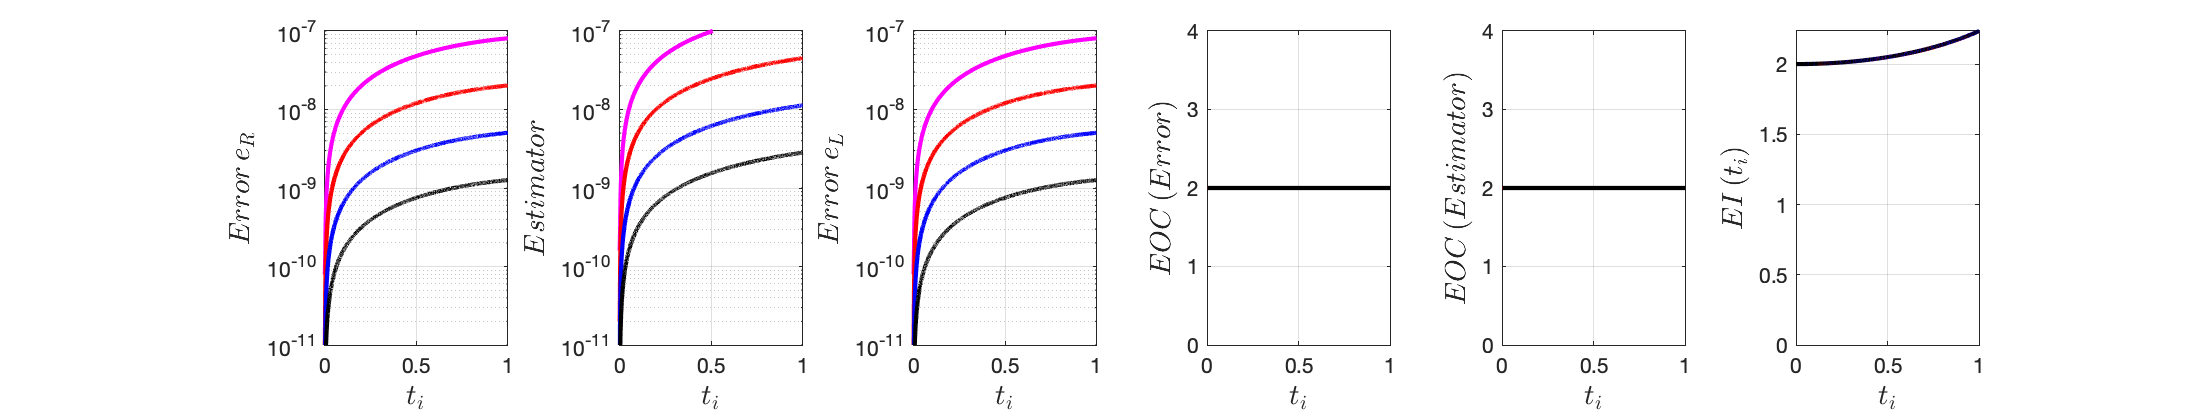
\includegraphics[scale=0.55]{fig_LeapFrogplots_1x5_sin_IC_harmonic_order_2_u0_v10_rec2}	
	\caption{Reconstruction from Defn. \ref{defn_our_rec2}. (from left to right) Error $e$ given by (\ref{eq_error_eR}), Estimator $\eta_1$ given by \ref{eq_bound_test}, EOC error, EOC Estimator, Effectivity Index.}
	\label{fig_all_in_one_our_rec_2_u0_v10}
\end{figure}

\begin{figure}[H]
	\hspace{-3cm}
	%\centering
	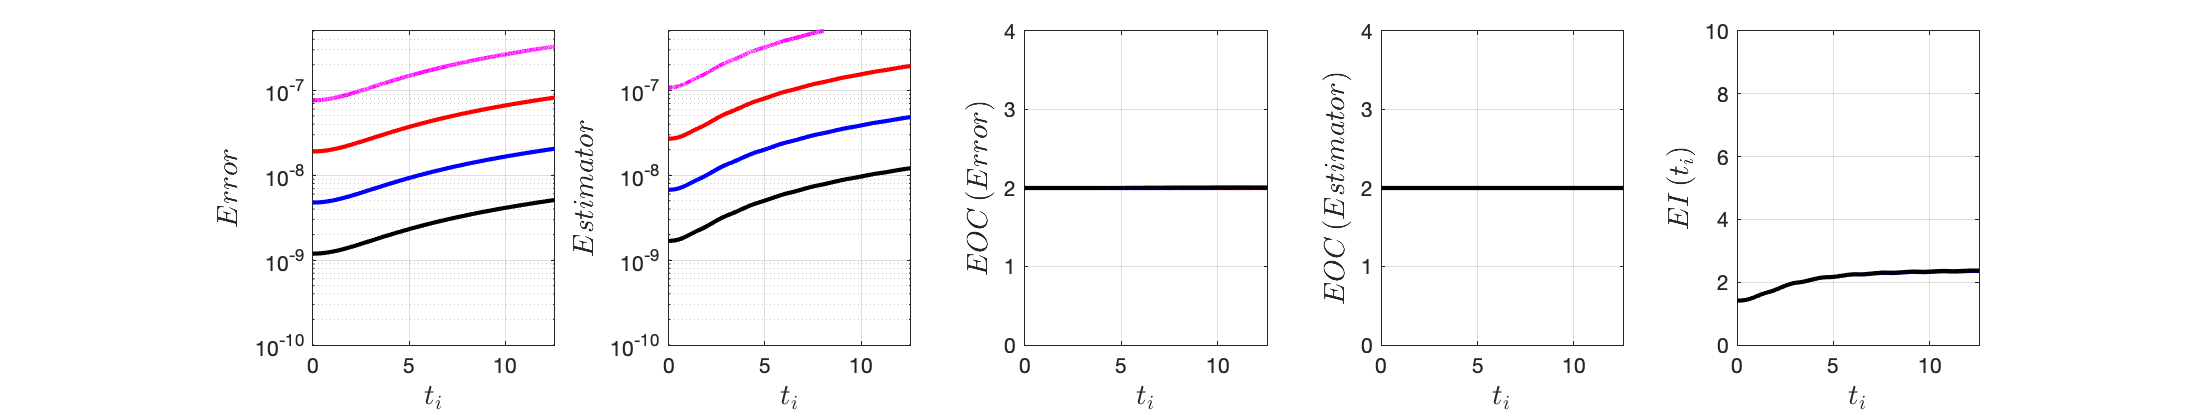
\includegraphics[scale=0.55]{fig_LeapFrogplots_1x5_sin_IC_harmonic_u0_v10_paperrec}	
	\caption{Paper rec. (from left to right) Error $e$ given by (\ref{eq_error_eR}), Estimator $\eta_1$ given by \ref{eq_bound_test}, EOC error, EOC Estimator, Effectivity Index.}
	\label{fig_all_in_one_paperrec_u0_v10}
\end{figure}
*/
\begin{figure}[H]
	\hspace{-3cm}
	%\centering
	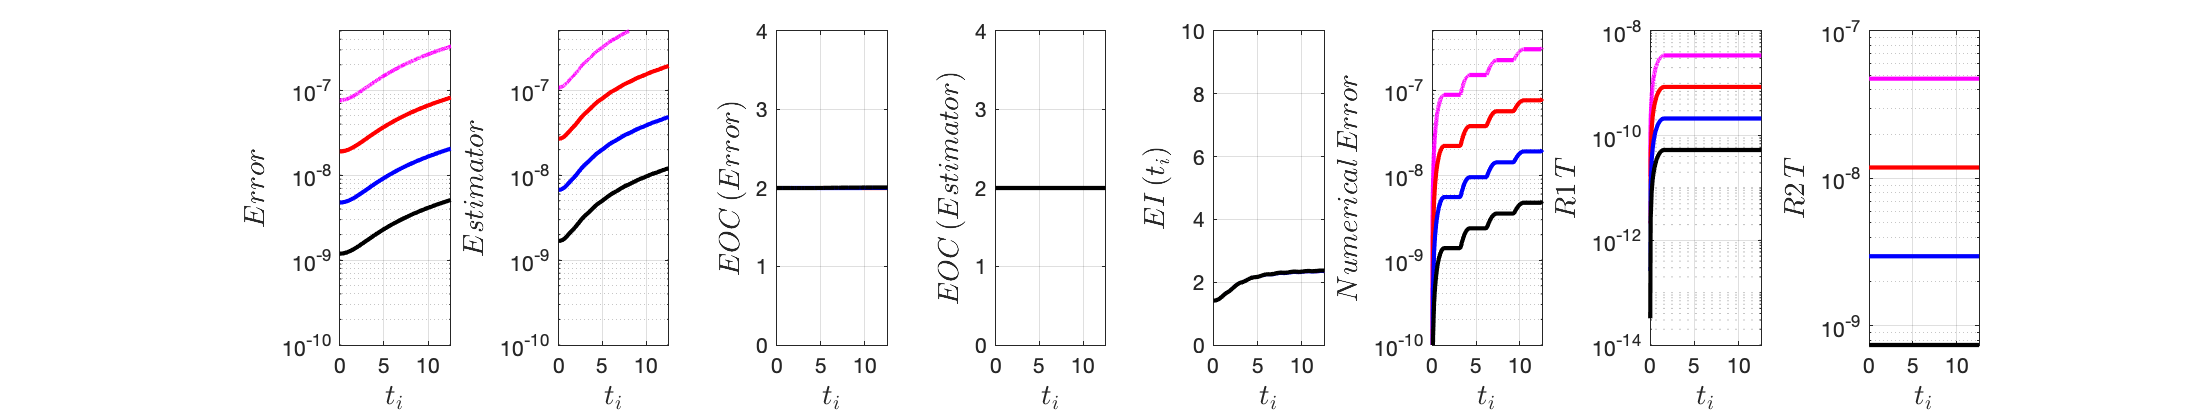
\includegraphics[scale=0.55]{fig_LeapFrogplots_1x5_sin_IC_harmonic_u0_v10_paperrec_poly_our_res}	
	\caption{Reconstruction from Defn. \ref{defn_rec_paper_poly}. (from left to right) Error $e$ given by (\ref{eq_error_eR}), Estimator $\eta_1$ given by (\ref{eq_bound_test}), EOC error, EOC Estimator, Effectivity Index.}
	\label{fig_all_in_one_paperrec_poly_u0_v10}
\end{figure}

\begin{figure}[H]
	\hspace{-3cm}
	%\centering
	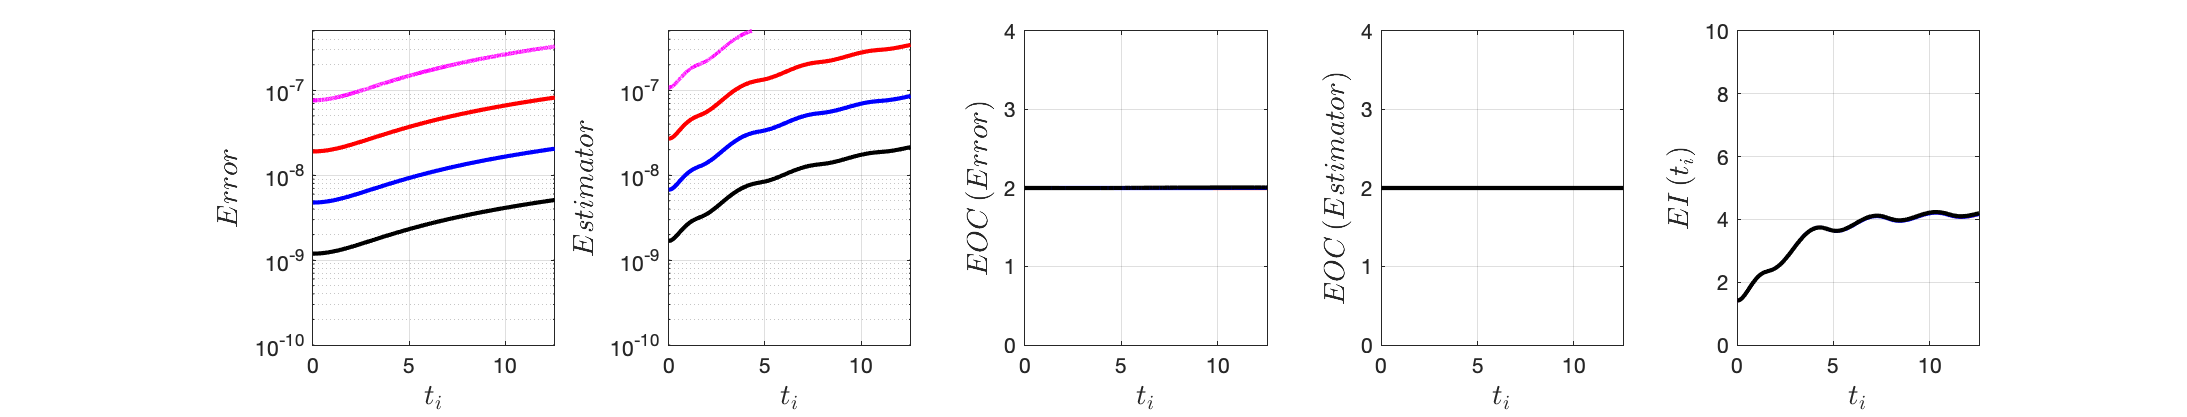
\includegraphics[scale=0.55]{fig_LeapFrogplots_1x5_sin_IC_harmonic_u0_v10_paperrec_poly_tristan}	
	\caption{Reconstruction from Defn. \ref{defn_our_rec3} (from left to right) Error $e$ given by (\ref{eq_error_eR}), Estimator $\eta_1$ given by (\ref{eq_bound_test}), EOC error, EOC Estimator, Effectivity Index.}
	\label{fig_all_in_one_paperrec_poly_tristan_u0_v10}
\end{figure}
\subsection*{$u_0=0.1, v_0= 0.9$}
\/*
\begin{figure}[H]
	\hspace{-3cm}
	%\centering
	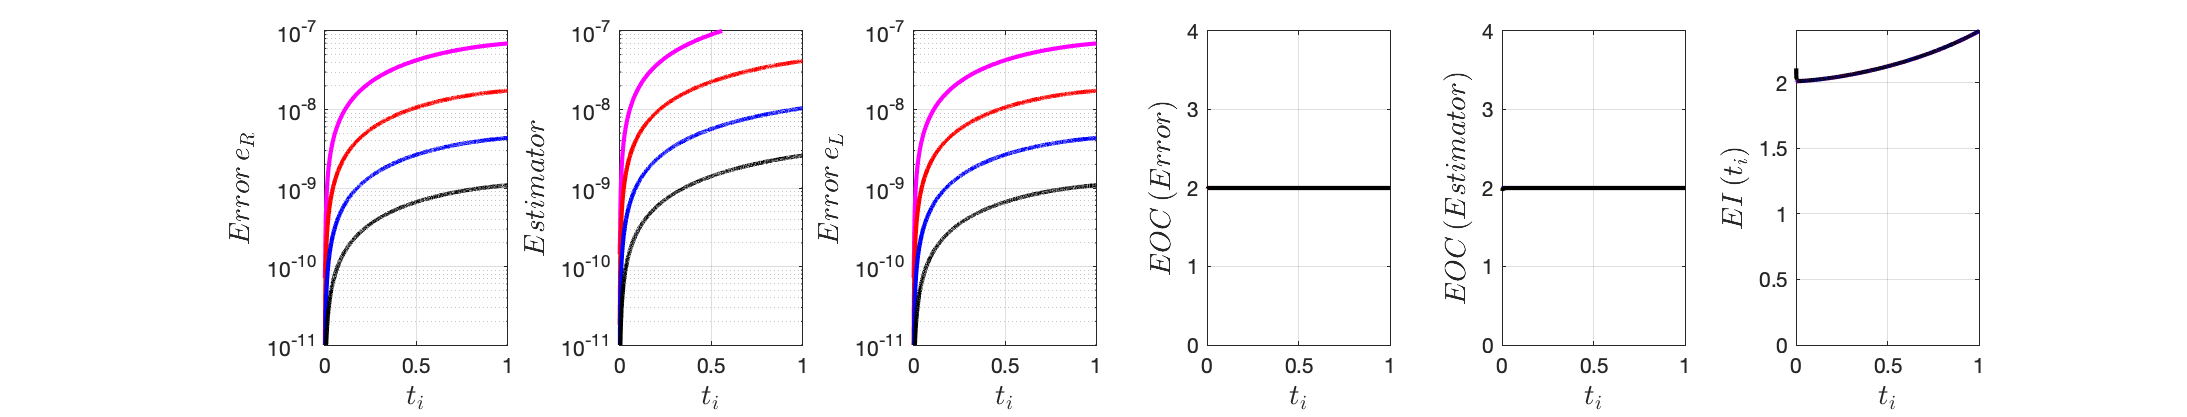
\includegraphics[scale=0.55]{fig_LeapFrogplots_1x5_sin_IC_harmonic_order_2_u1_v9_rec_george}	
	\caption{Reconstruction from Defn. \ref{defn_our_rec}. (from left to right) Error $e$ given by (\ref{eq_error_eR}), Estimator $\eta_1$ given by \ref{eq_bound_test},  EOC error, EOC Estimator, Effectivity Index.}
	\label{fig_all_in_one_our_rec_george_u1_v9}
\end{figure}

\begin{figure}[H]
	\hspace{-3cm}
	%\centering
	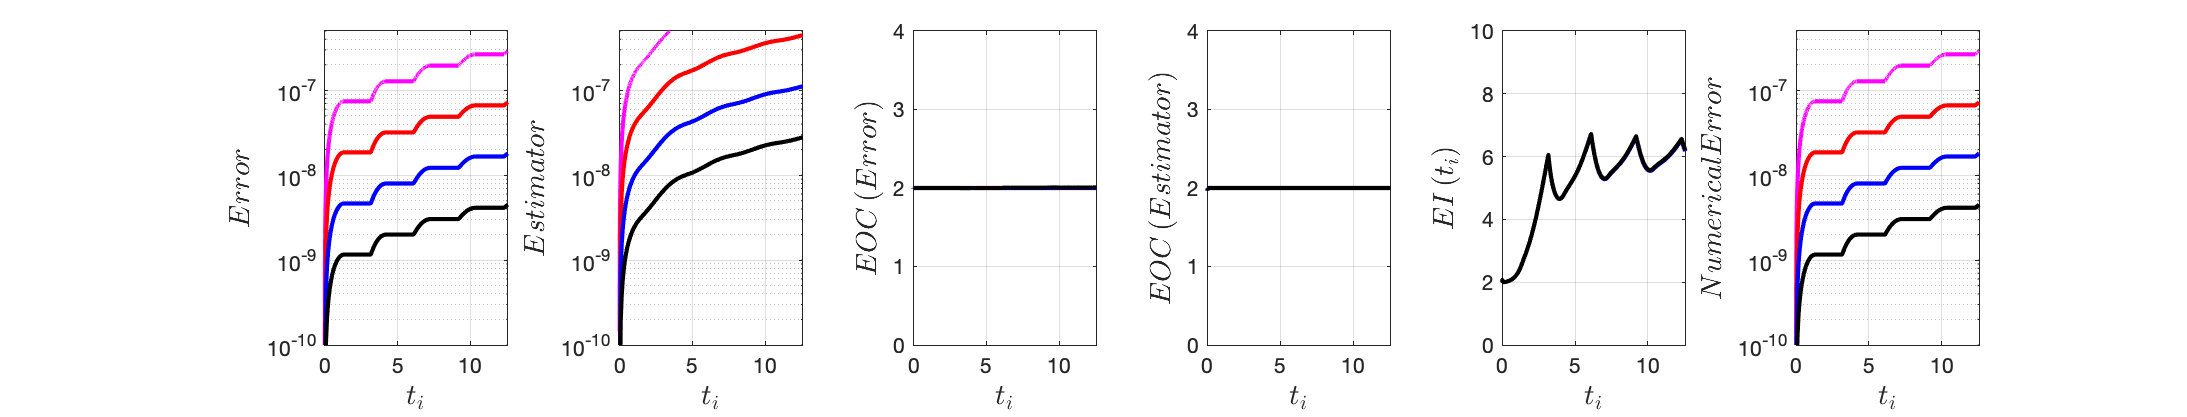
\includegraphics[scale=0.55]{fig_LeapFrogplots_1x5_sin_IC_harmonic_order_2_u1_v9_rec2}	
	\caption{Reconstruction from Defn. \ref{defn_our_rec2}. (from left to right) Error $e$ given by (\ref{eq_error_eR}), Estimator $\eta_1$ given by \ref{eq_bound_test},  EOC error, EOC Estimator, Effectivity Index.}
	\label{fig_all_in_one_our_rec_2_u1_v9}
\end{figure}
\begin{figure}[H]
	\hspace{-3cm}
	%\centering
	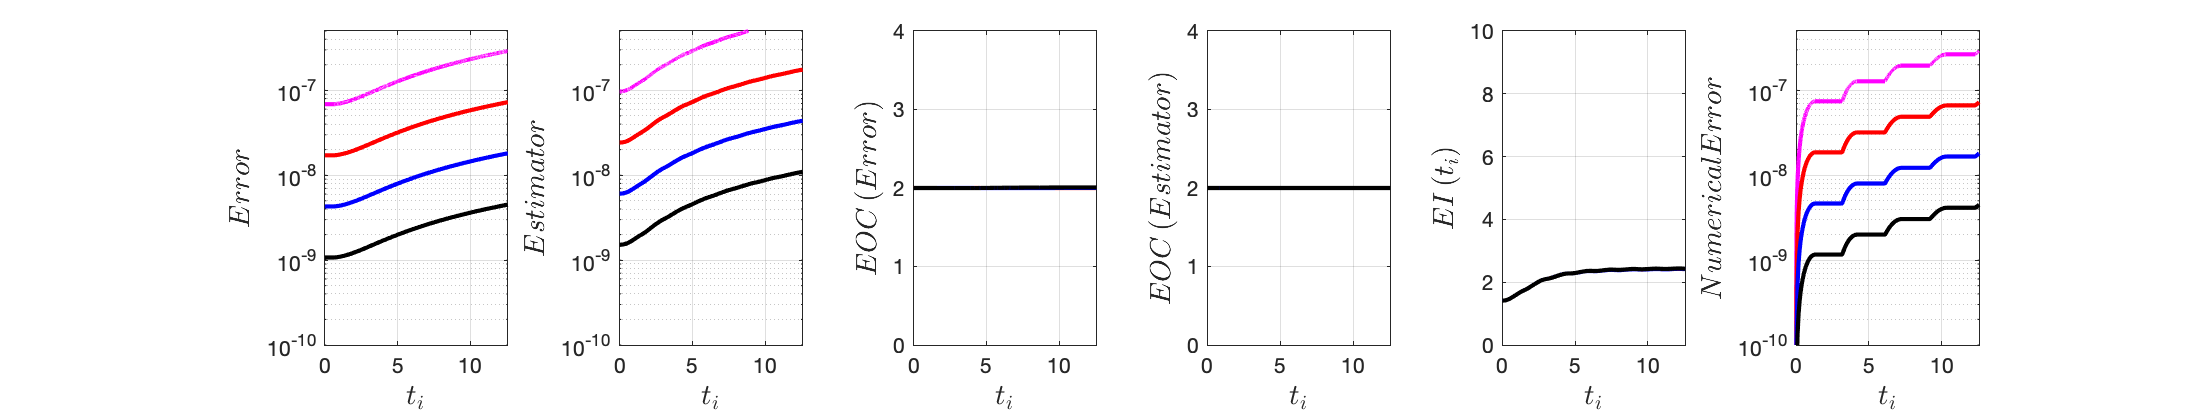
\includegraphics[scale=0.55]{fig_LeapFrogplots_1x5_sin_IC_harmonic_u1_v9_paperrec}	
	\caption{Paper rec. (from left to right) Error $e$ given by (\ref{eq_error_eR}), Estimator $\eta_1$ given by \ref{eq_bound_test},  EOC error, EOC Estimator, Effectivity Index.}
	\label{fig_all_in_one_paperrec_u01_v09}
\end{figure}
*/

\begin{figure}[H]
	\hspace{-3cm}
	%\centering
	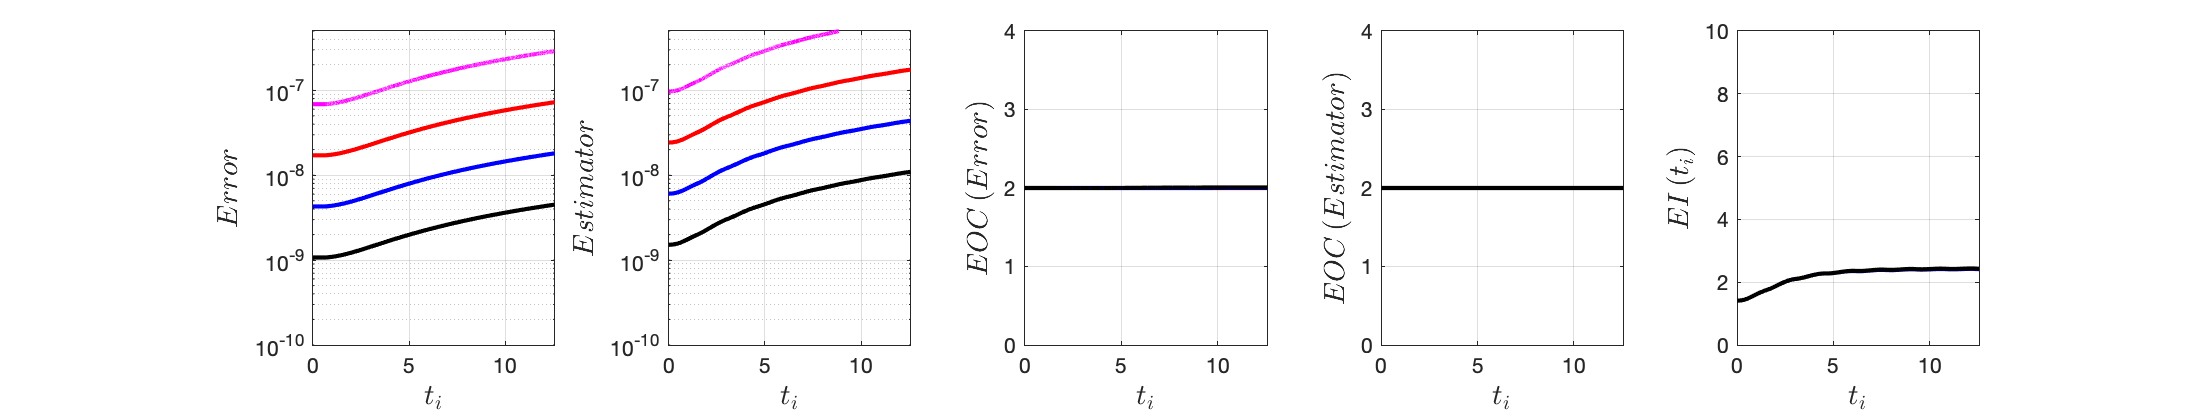
\includegraphics[scale=0.55]{fig_LeapFrogplots_1x5_sin_IC_harmonic_u1_v9_paperrec_poly_our_res}	
		\caption{Reconstruction from Defn. \ref{defn_rec_paper_poly}. (from left to right) Error $e$ given by (\ref{eq_error_eR}), Estimator $\eta_1$ given by (\ref{eq_bound_test}), EOC error, EOC Estimator, Effectivity Index.}
	\label{fig_all_in_one_paperrec_poly_u01_v09}
\end{figure}
\begin{figure}[H]
	\hspace{-3cm}
	%\centering
	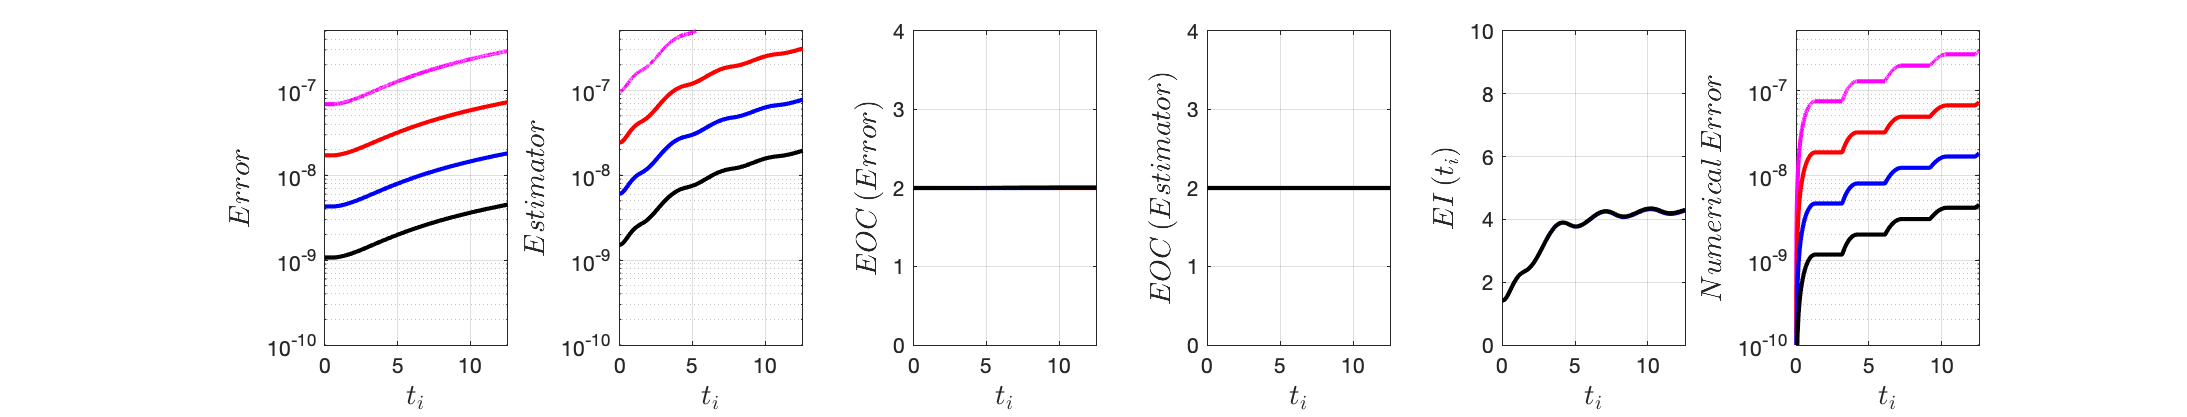
\includegraphics[scale=0.55]{fig_LeapFrogplots_1x5_sin_IC_harmonic_u1_v9_paperrec_poly_tristan}	
	\caption{Polynomial  rec. from Defn. \ref{defn_our_rec3} (from left to right) Error $e$ given by (\ref{eq_error_eR}), Estimator $\eta_1$ given by \ref{eq_bound_test}, EOC error, EOC Estimator, Effectivity Index.}
	\label{fig_all_in_one_paperrec_poly_tristan_u1_v9}
\end{figure}


\subsection*{$u_0=0.2, v_0= 0.8$}
\/*
\begin{figure}[H]
	\hspace{-3cm}
	%\centering
	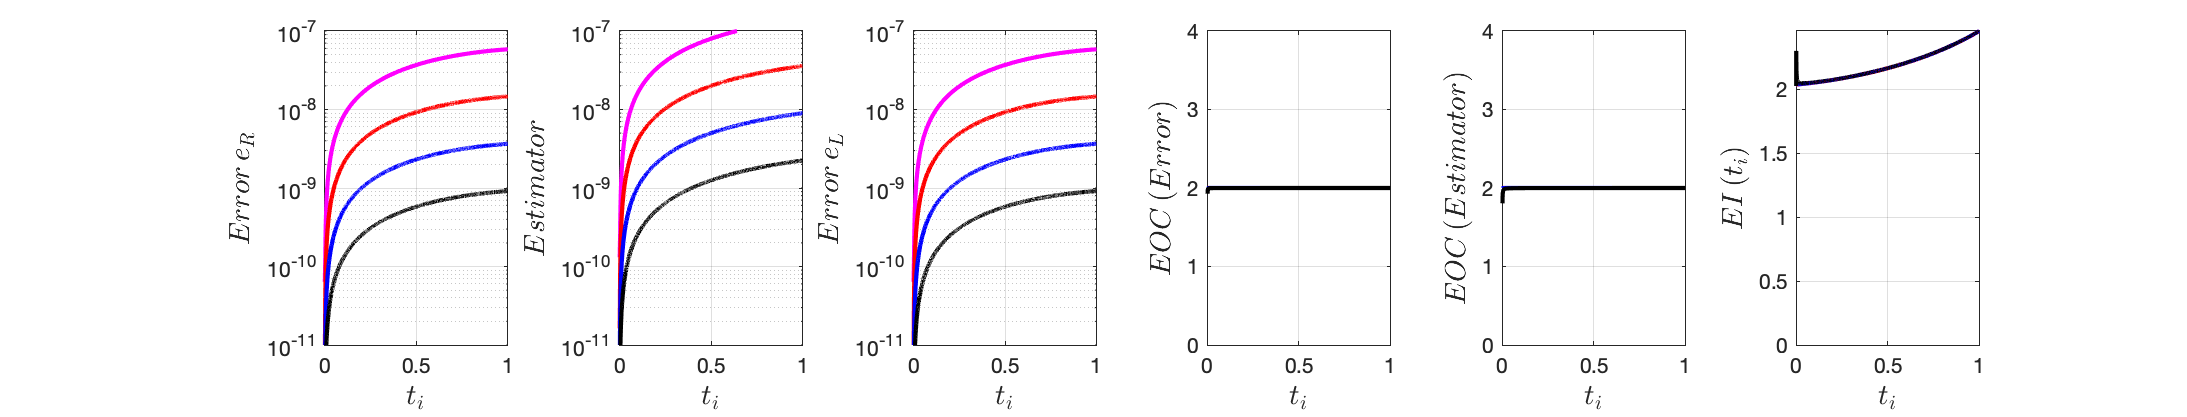
\includegraphics[scale=0.55]{fig_LeapFrogplots_1x5_sin_IC_harmonic_order_2_u2_v8_rec_george}	
	\caption{Reconstruction from Defn. \ref{defn_our_rec}. (from left to right) Error $e$ given by (\ref{eq_error_eR}), Estimator $\eta_1$ given by \ref{eq_bound_test},  EOC error, EOC Estimator, Effectivity Index.}
	\label{fig_all_in_one_our_rec_george_u2_v8}
\end{figure}
\begin{figure}[H]
	\hspace{-3cm}
	%\centering
	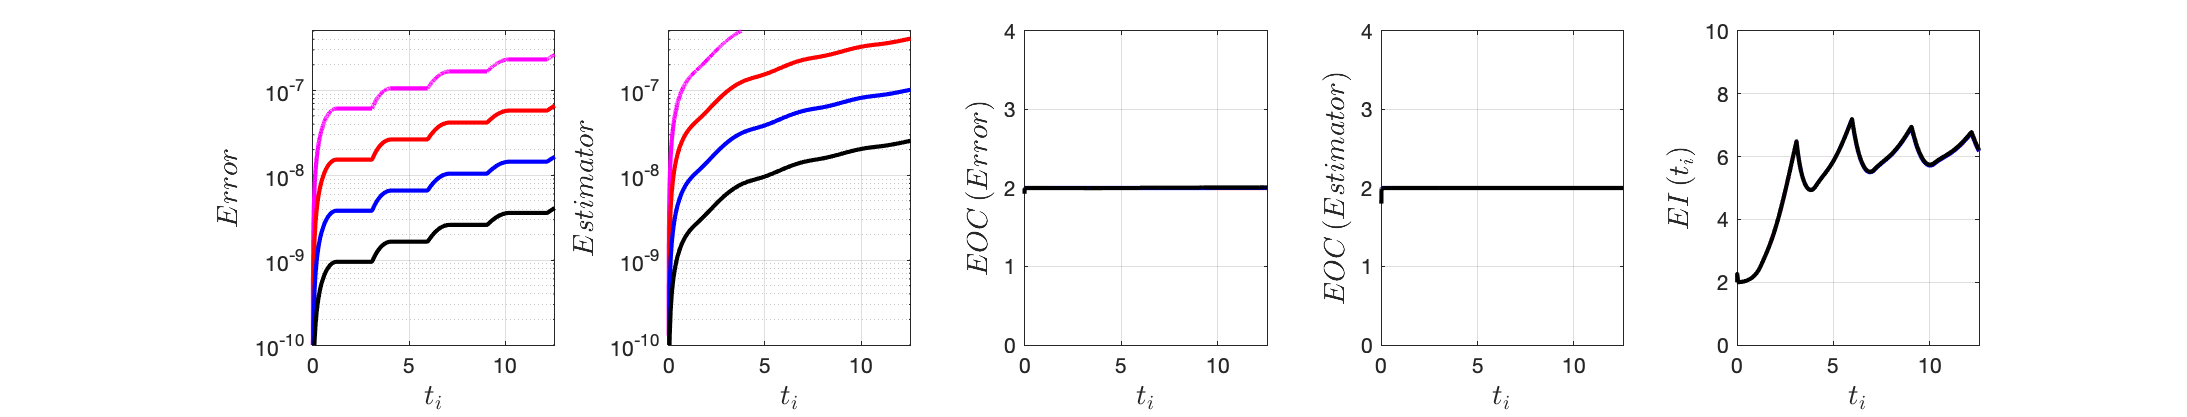
\includegraphics[scale=0.55]{fig_LeapFrogplots_1x5_sin_IC_harmonic_order_2_u2_v8_rec2}	
	\caption{Reconstruction from Defn. \ref{defn_our_rec2}. (from left to right) Error $e$ given by (\ref{eq_error_eR}), Estimator $\eta_1$ given by \ref{eq_bound_test},   EOC error, EOC Estimator, Effectivity Index.}
	\label{fig_all_in_one_our_rec_2_u2_v8}
\end{figure}

\begin{figure}[H]
	\hspace{-3cm}
	%\centering
	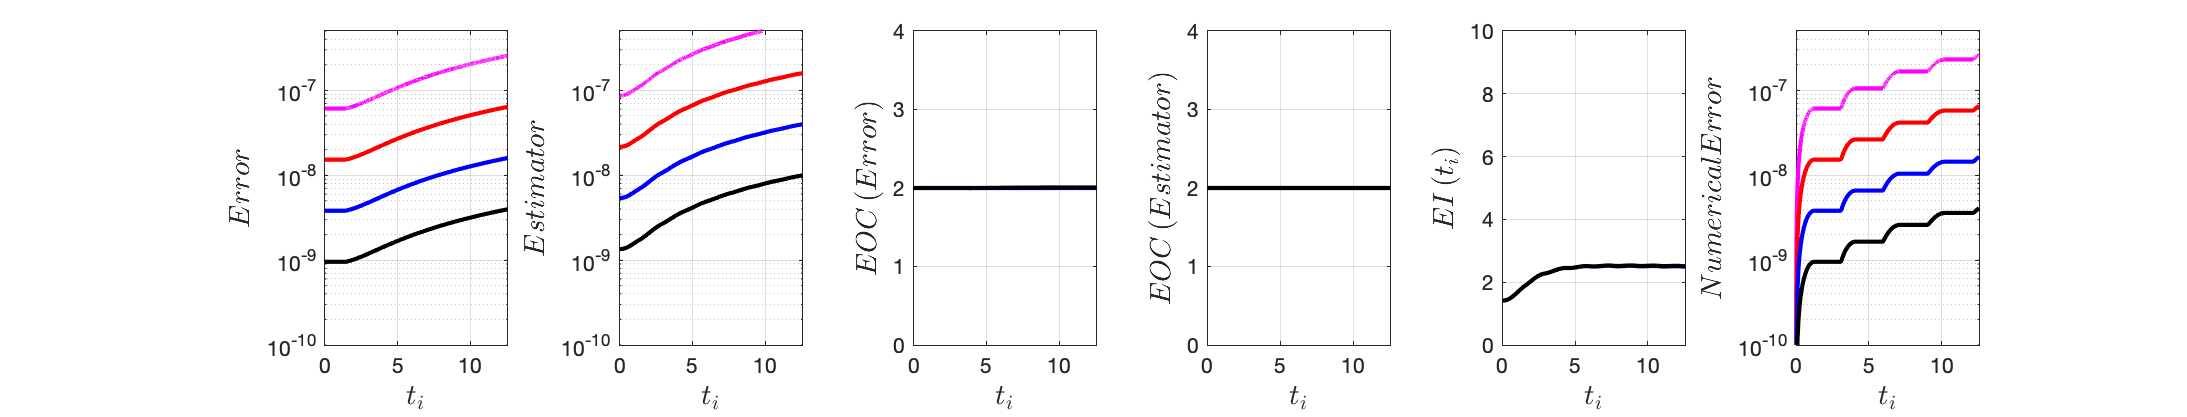
\includegraphics[scale=0.55]{fig_LeapFrogplots_1x5_sin_IC_harmonic_u2_v8_paperrec}	
	\caption{Paper rec. (from left to right) Error $e$ given by (\ref{eq_error_eR}), Estimator $\eta_1$ given by \ref{eq_bound_test},   EOC error, EOC Estimator, Effectivity Index.}
	\label{fig_all_in_one_paperrec_u02_v08}
\end{figure}
*/
\begin{figure}[H]
	\hspace{-3cm}
	%\centering
	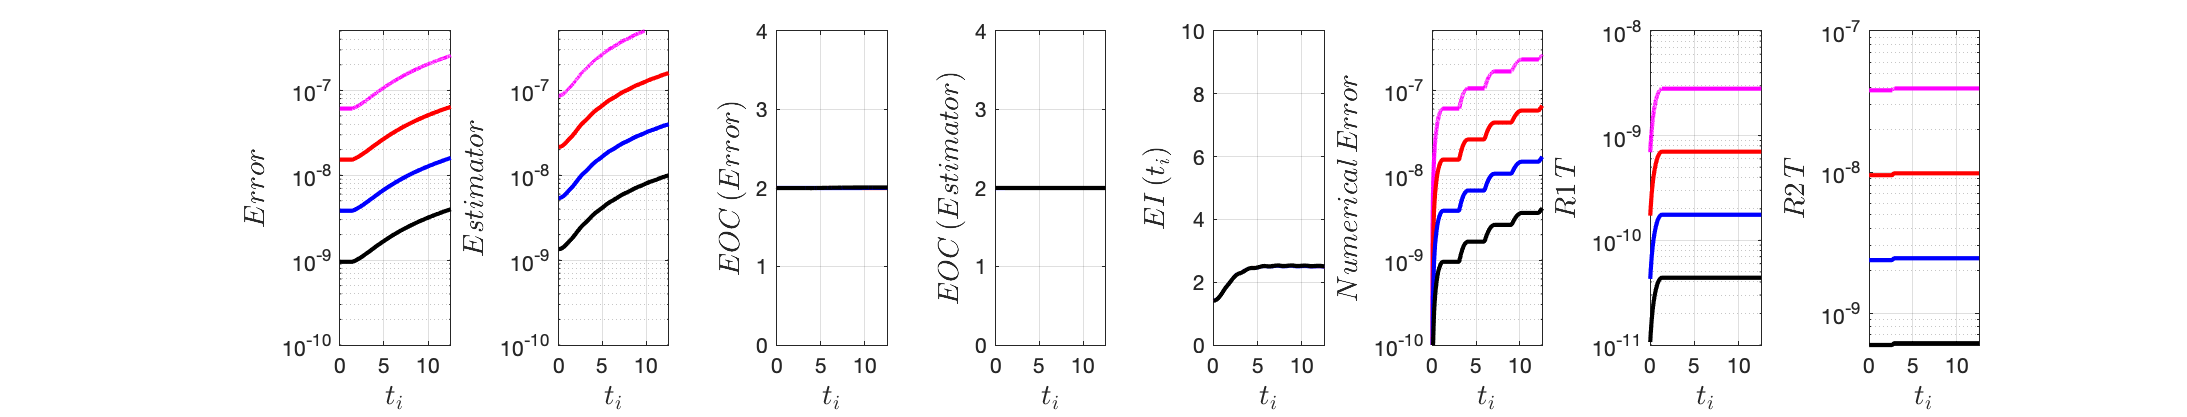
\includegraphics[scale=0.55]{fig_LeapFrogplots_1x5_sin_IC_harmonic_u2_v8_paperrec_poly_our_res}	
		\caption{Reconstruction from Defn. \ref{defn_rec_paper_poly}. (from left to right) Error $e$ given by (\ref{eq_error_eR}), Estimator $\eta_1$ given by (\ref{eq_bound_test}), EOC error, EOC Estimator, Effectivity Index.}
	\label{fig_all_in_one_paperrec_poly_u02_v08}
\end{figure}

\begin{figure}[H]
	\hspace{-3cm}
	%\centering
	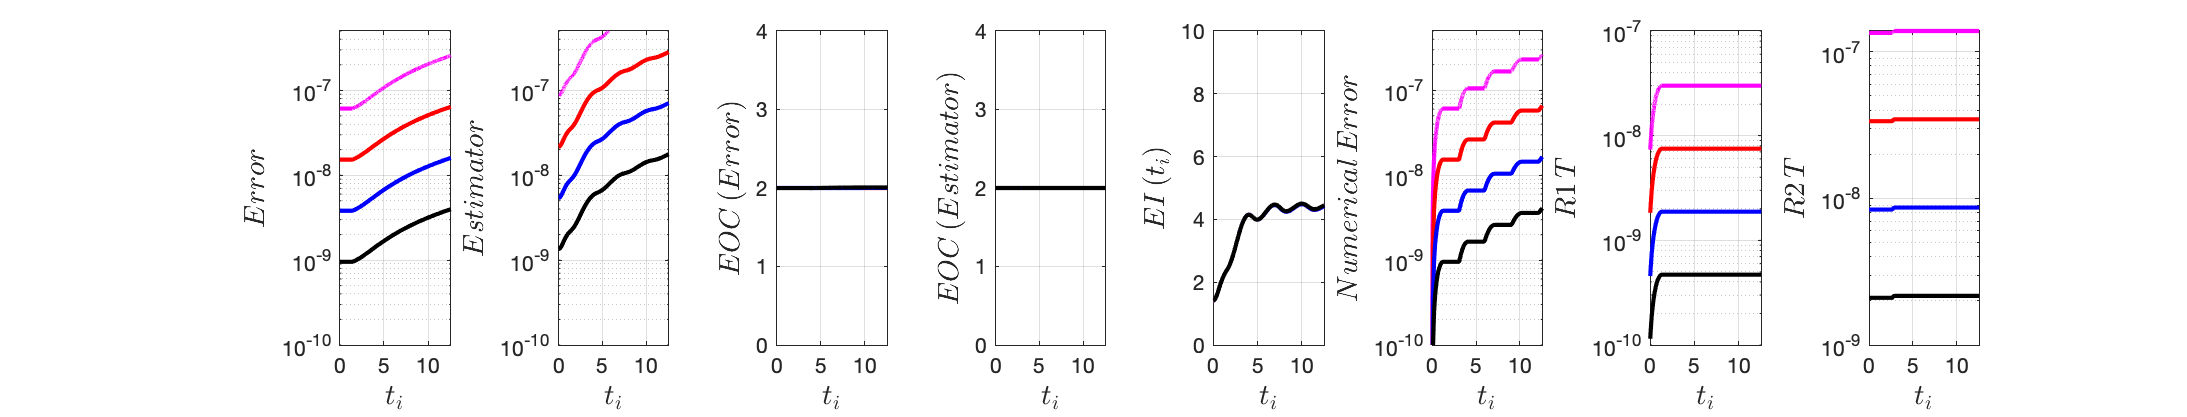
\includegraphics[scale=0.55]{fig_LeapFrogplots_1x5_sin_IC_harmonic_u2_v8_paperrec_poly_tristan}	
	\caption{Reconstruction from Defn. \ref{defn_our_rec3} (from left to right) Error $e$ given by (\ref{eq_error_eR}), Estimator $\eta_1$ given by (\ref{eq_bound_test}), EOC error, EOC Estimator, Effectivity Index.}
	\label{fig_all_in_one_paperrec_poly_tristan_u2_v8}
\end{figure}

\subsection*{$u_0=0.3, v_0= 0.7$}
\/*
\begin{figure}[H]
	\hspace{-3cm}
	%\centering
	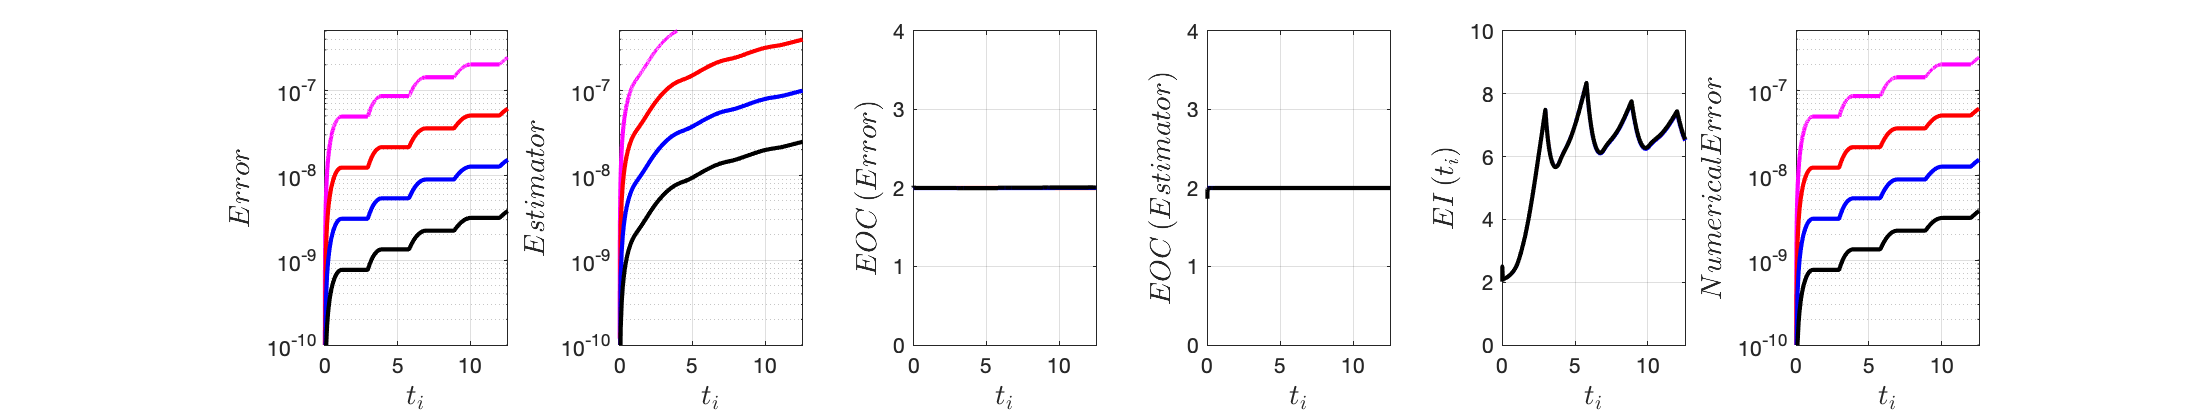
\includegraphics[scale=0.55]{fig_LeapFrogplots_1x5_sin_IC_harmonic_order_2_u3_v7_rec_george}	
	\caption{Reconstruction from Defn. \ref{defn_our_rec}. (from left to right) Error $e$ given by (\ref{eq_error_eR}), Estimator $\eta_1$ given by \ref{eq_bound_test},   EOC error, EOC Estimator, Effectivity Index.}
	\label{fig_all_in_one_our_rec_george_u3_v7}
\end{figure}
\begin{figure}[H]
	\hspace{-3cm}
	%\centering
	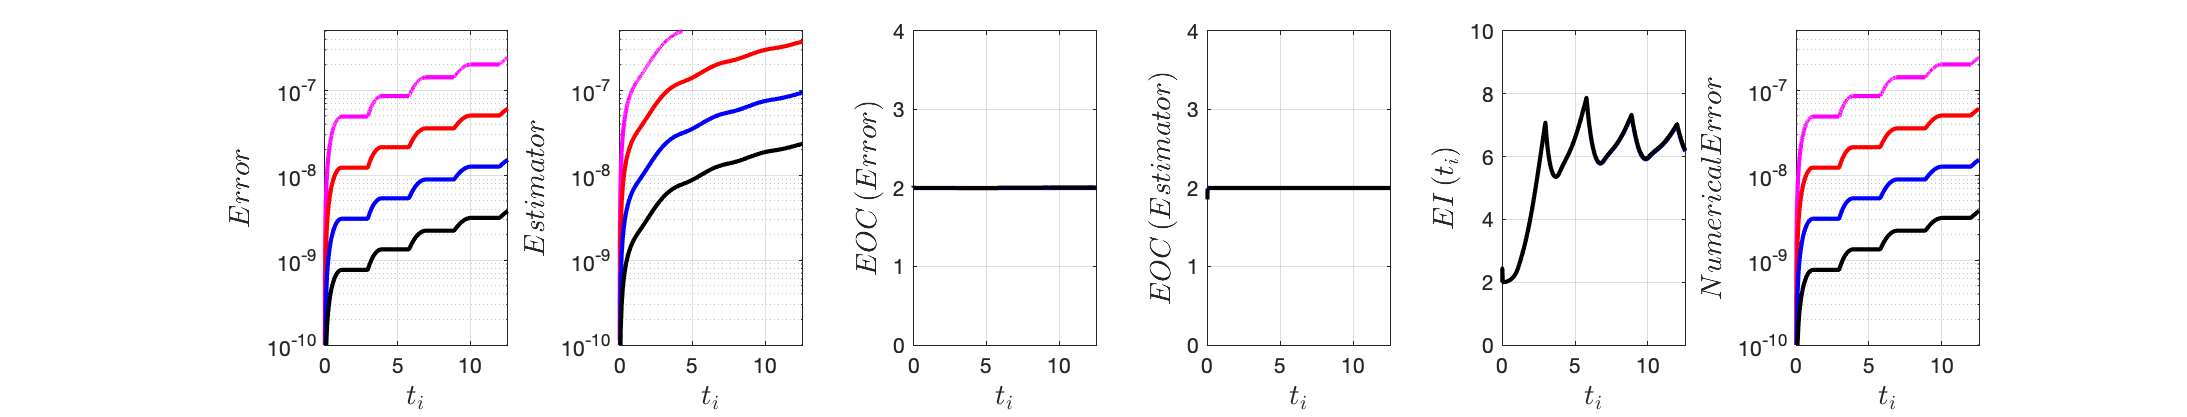
\includegraphics[scale=0.55]{fig_LeapFrogplots_1x5_sin_IC_harmonic_order_2_u3_v7_rec2}	
	\caption{Reconstruction from Defn. \ref{defn_our_rec2}. (from left to right) Error $e$ given by (\ref{eq_error_eR}), Estimator $\eta_1$ given by \ref{eq_bound_test},  EOC error, EOC Estimator, Effectivity Index.}
	\label{fig_all_in_one_our_rec_2_u3_v7}
\end{figure}
\begin{figure}[H]
	\hspace{-3cm}
	%\centering
	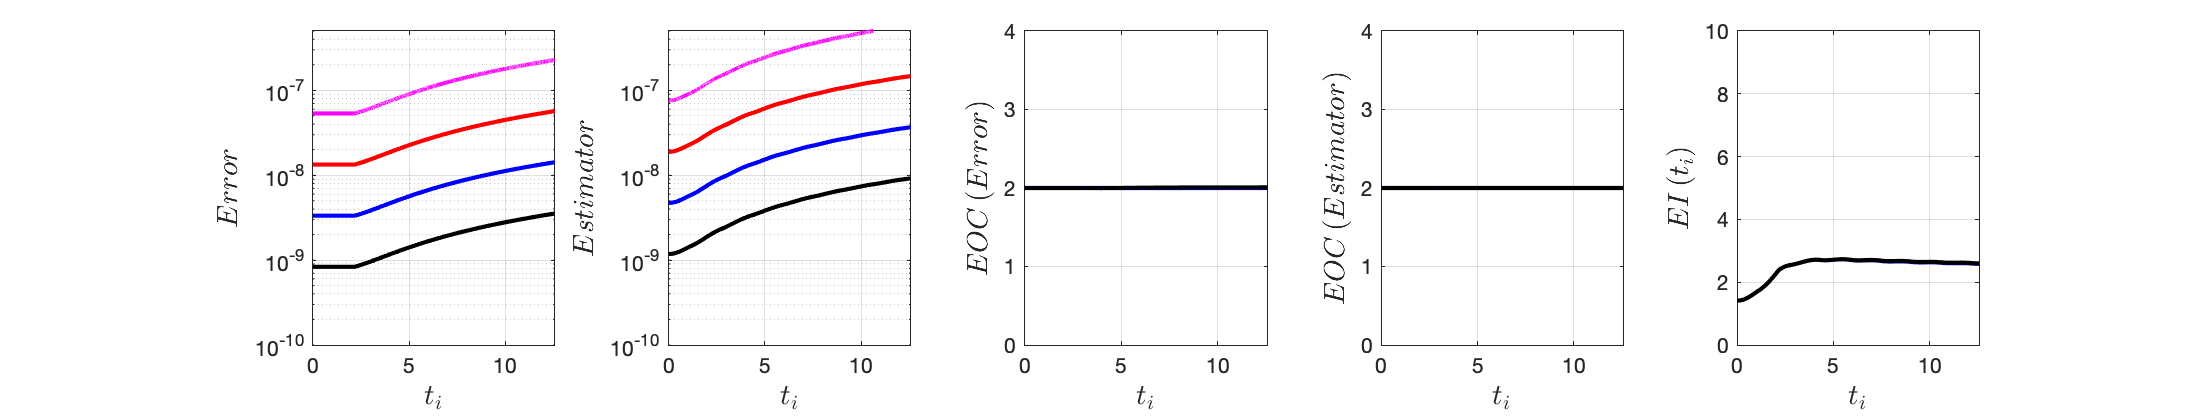
\includegraphics[scale=0.55]{fig_LeapFrogplots_1x5_sin_IC_harmonic_u3_v7_paperrec}	
	\caption{Paper rec. (from left to right) Error $e$ given by (\ref{eq_error_eR}), Estimator $\eta_1$ given by \ref{eq_bound_test}, EOC error, EOC Estimator, Effectivity Index.}
	\label{fig_all_in_one_paperrec_u03_v07}
\end{figure}
*/
\begin{figure}[H]
	\hspace{-3cm}
	%\centering
	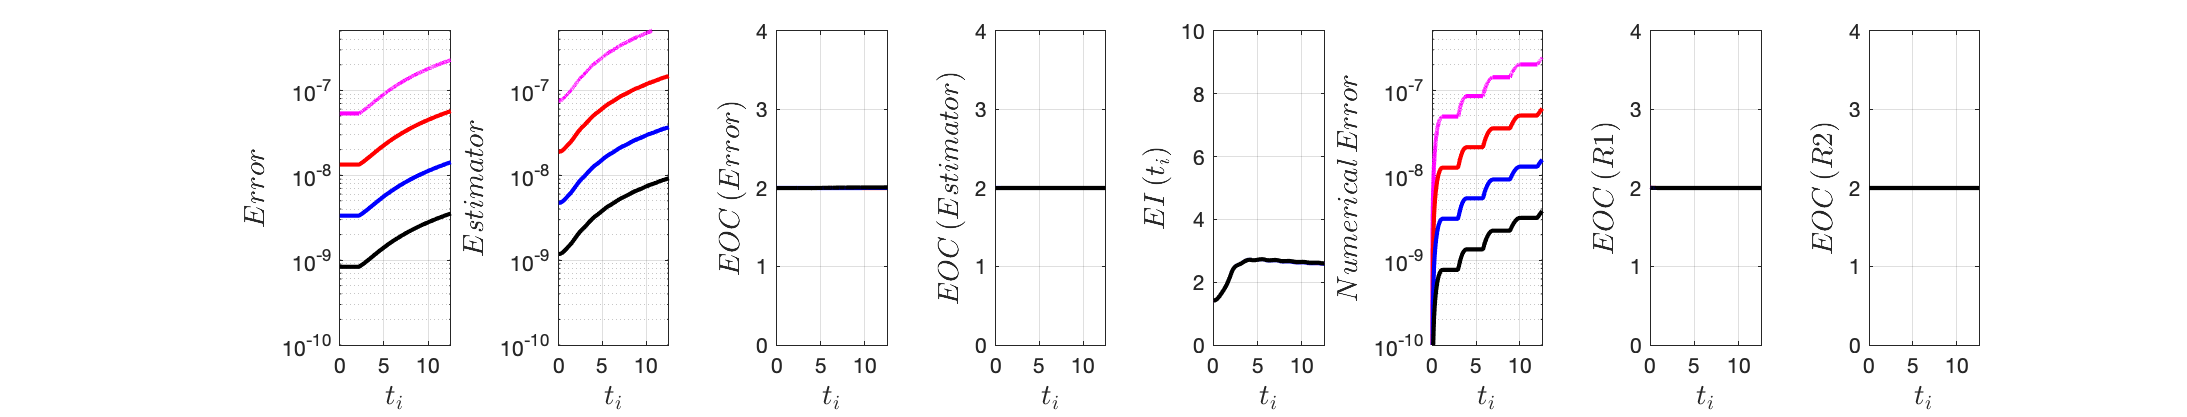
\includegraphics[scale=0.55]{fig_LeapFrogplots_1x5_sin_IC_harmonic_u3_v7_paperrec_poly_our_res}	
		\caption{Reconstruction from Defn. \ref{defn_rec_paper_poly}. (from left to right) Error $e$ given by (\ref{eq_error_eR}), Estimator $\eta_1$ given by (\ref{eq_bound_test}), EOC error, EOC Estimator, Effectivity Index.}
	\label{fig_all_in_one_paperrec_polynomial_u03_v07}
\end{figure}

\begin{figure}[H]
	\hspace{-3cm}
	%\centering
	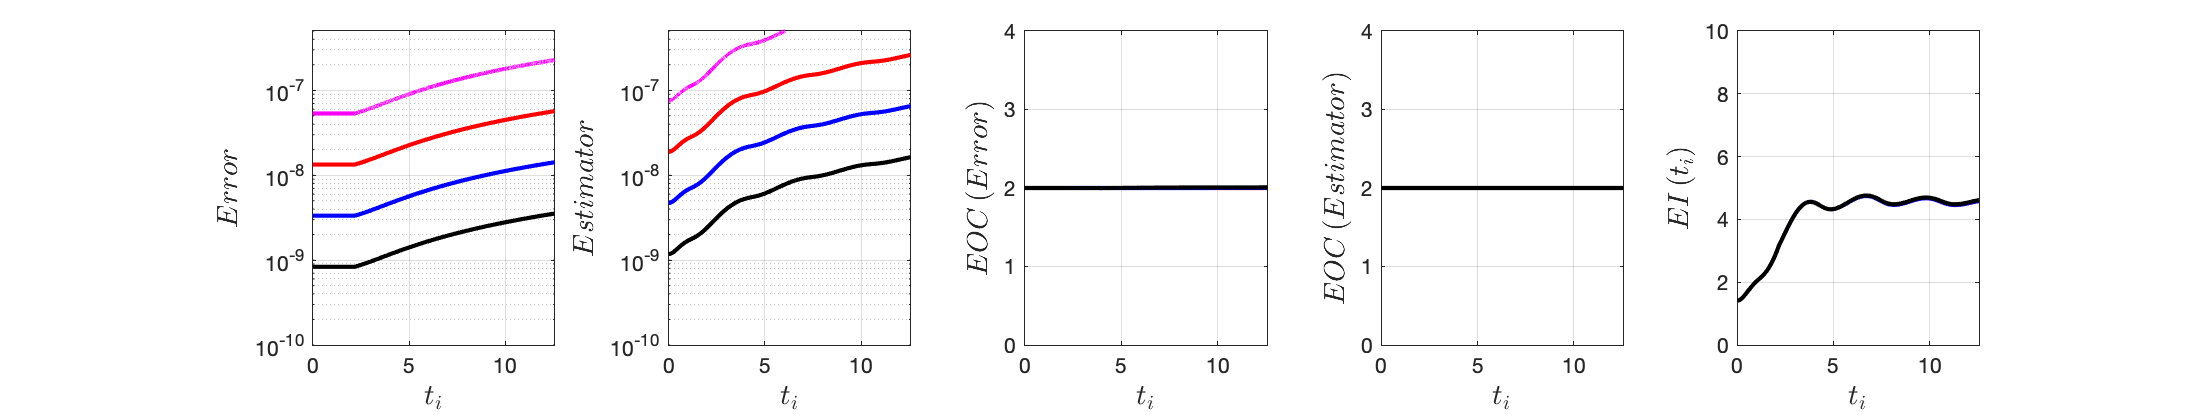
\includegraphics[scale=0.55]{fig_LeapFrogplots_1x5_sin_IC_harmonic_u3_v7_paperrec_poly_tristan}	
	\caption{Reconstruction from Defn. \ref{defn_our_rec3} (from left to right) Error $e$ given by (\ref{eq_error_eR}), Estimator $\eta_1$ given by (\ref{eq_bound_test}), EOC error, EOC Estimator, Effectivity Index.}
	\label{fig_all_in_one_paperrec_poly_tristan_u3_v7}
\end{figure}

\subsection*{$u_0=0.4, v_0= 0.6$}
\/*
\begin{figure}[H]
	\hspace{-3cm}
	%\centering
	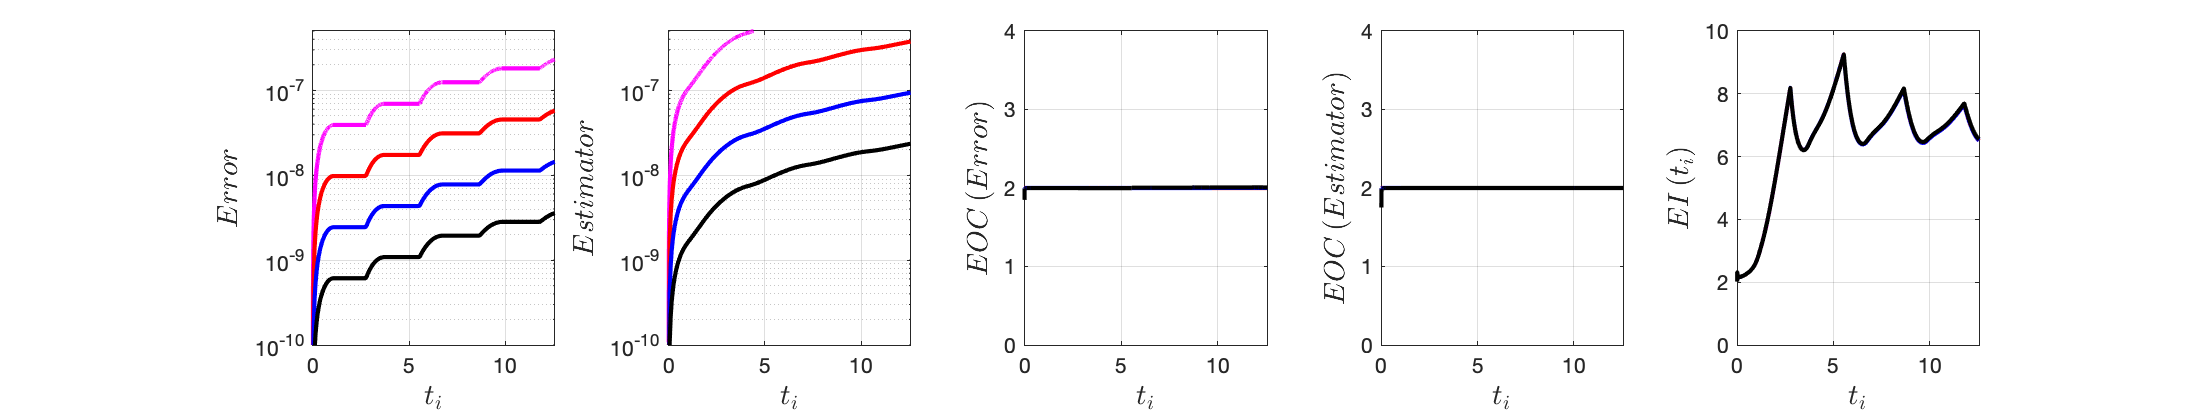
\includegraphics[scale=0.55]{fig_LeapFrogplots_1x5_sin_IC_harmonic_order_2_u4_v6_rec_george}	
	\caption{Reconstruction from Defn. \ref{defn_our_rec}. (from left to right) Error $e$ given by (\ref{eq_error_eR}), Estimator $\eta_1$ given by \ref{eq_bound_test},  EOC error, EOC Estimator, Effectivity Index.}
	\label{fig_all_in_one_our_rec_george_u4_v6}
\end{figure}
\begin{figure}[H]
	\hspace{-3cm}
	%\centering
	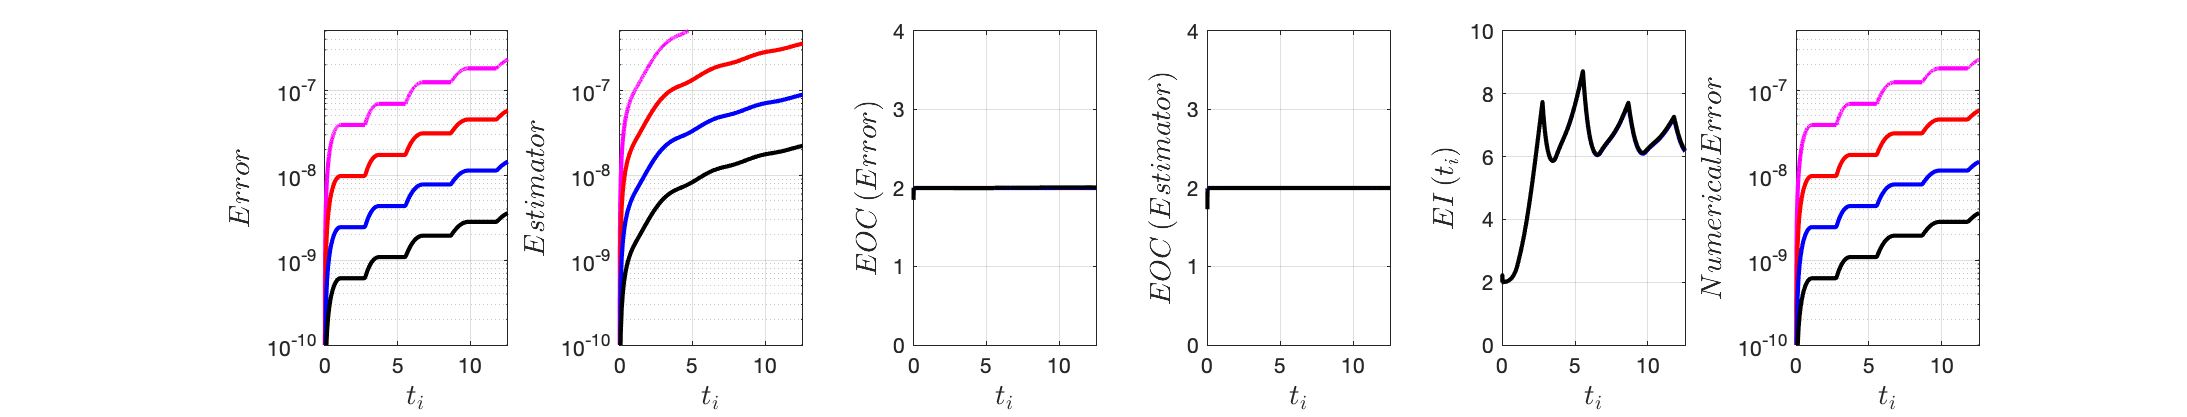
\includegraphics[scale=0.55]{fig_LeapFrogplots_1x5_sin_IC_harmonic_order_2_u4_v6_rec2}	
	\caption{Reconstruction from Defn. \ref{defn_our_rec2}. (from left to right) Error $e$ given by (\ref{eq_error_eR}), Estimator $\eta_1$ given by \ref{eq_bound_test},  EOC error, EOC Estimator, Effectivity Index.}
	\label{fig_all_in_one_our_rec_2_u4_v6}
\end{figure}
\begin{figure}[H]
	\hspace{-3cm}
	%\centering
	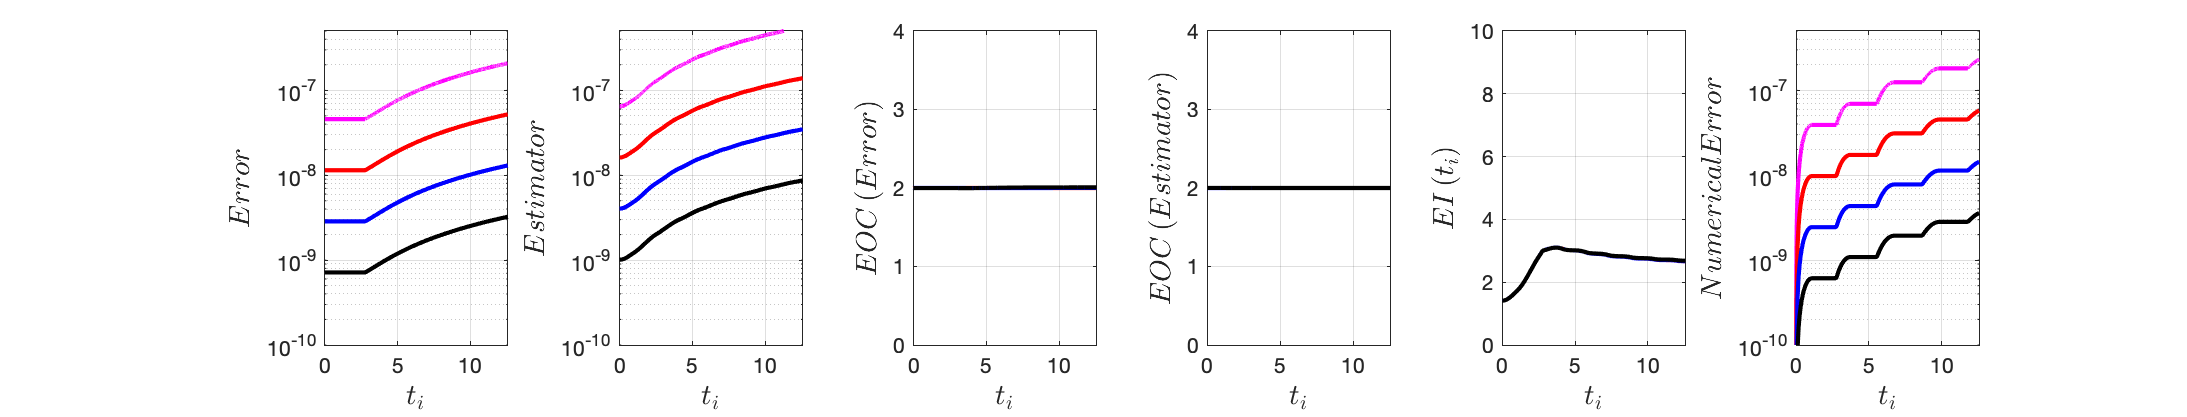
\includegraphics[scale=0.55]{fig_LeapFrogplots_1x5_sin_IC_harmonic_u4_v6_paperrec}	
	\caption{Paper rec. (from left to right) Error $e$ given by (\ref{eq_error_eR}), Estimator $\eta_1$ given by \ref{eq_bound_test},  EOC error, EOC Estimator, Effectivity Index.}
	\label{fig_all_in_one_paperrec_u04_v06}
\end{figure}
*/
\begin{figure}[H]
	\hspace{-3cm}
	%\centering
	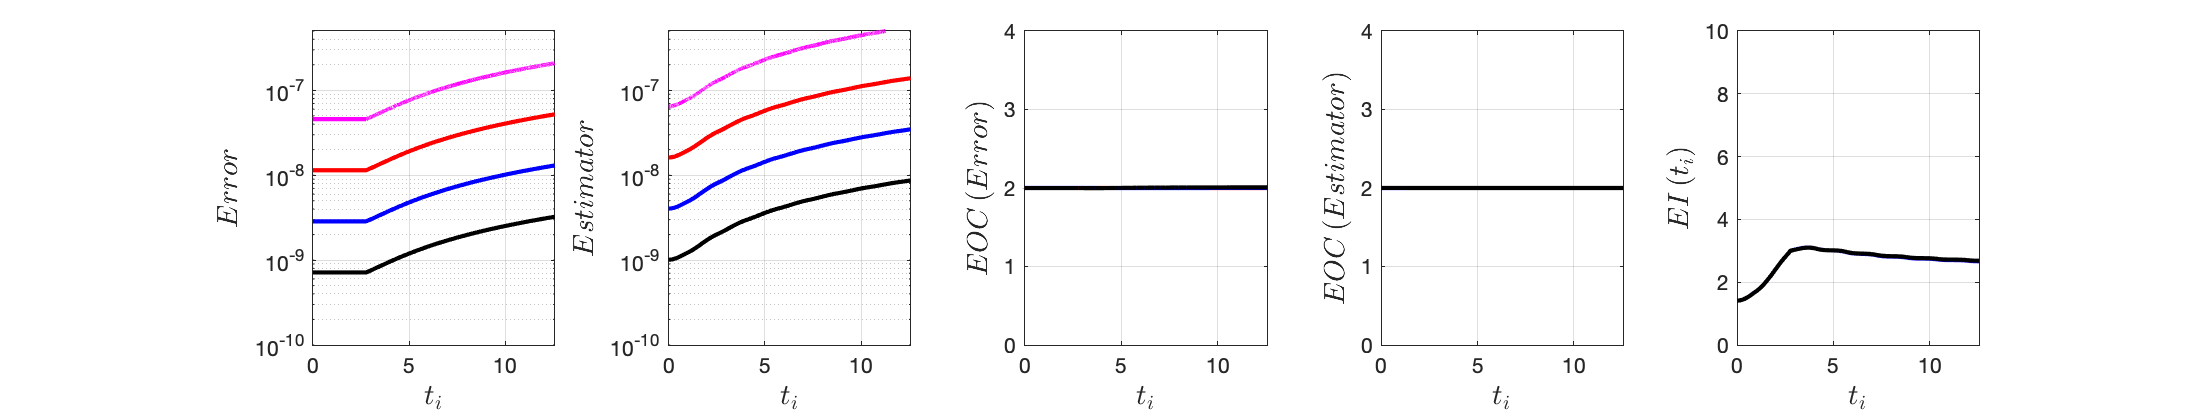
\includegraphics[scale=0.55]{fig_LeapFrogplots_1x5_sin_IC_harmonic_u4_v6_paperrec_poly_our_res}	
	\caption{Reconstruction from Defn. \ref{defn_rec_paper_poly}. (from left to right) Error $e$ given by (\ref{eq_error_eR}), Estimator $\eta_1$ given by (\ref{eq_bound_test}), EOC error, EOC Estimator, Effectivity Index.}
	\label{fig_all_in_one_paperrec_poly_u04_v06}
\end{figure}

\begin{figure}[H]
	\hspace{-3cm}
	%\centering
	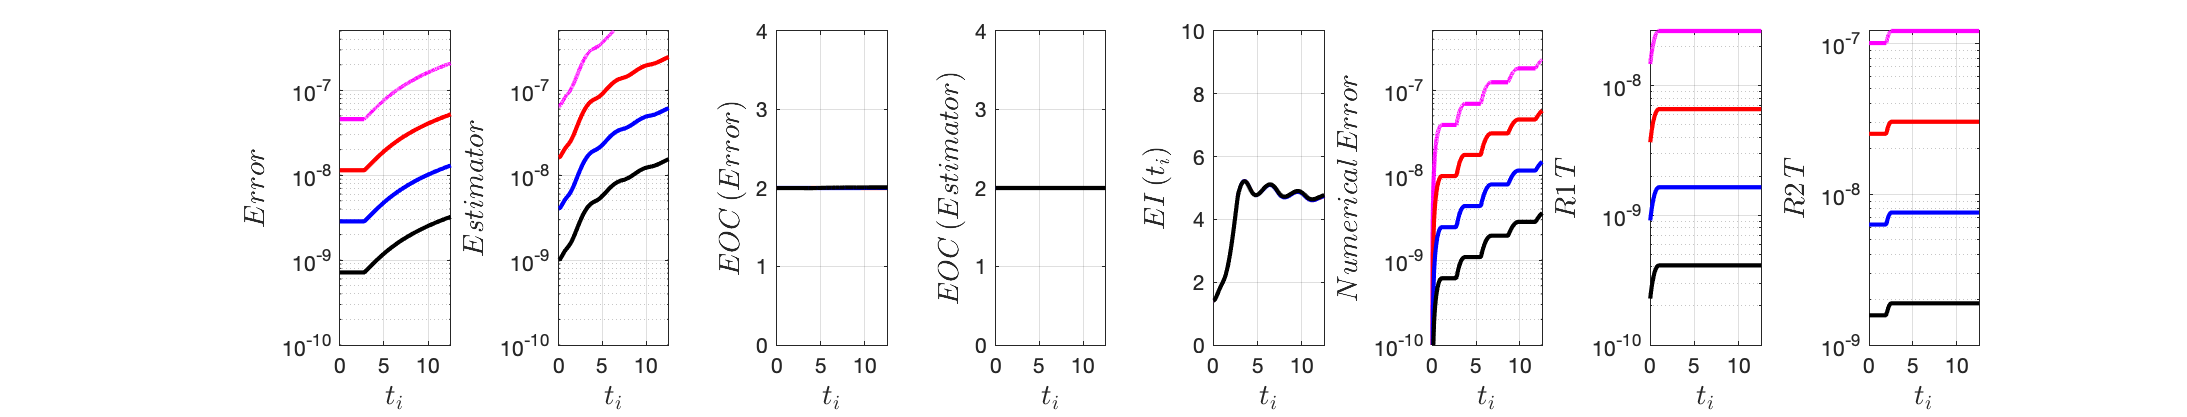
\includegraphics[scale=0.55]{fig_LeapFrogplots_1x5_sin_IC_harmonic_u4_v6_paperrec_poly_tristan}	
\caption{Reconstruction from Defn. \ref{defn_our_rec3} (from left to right) Error $e$ given by (\ref{eq_error_eR}), Estimator $\eta_1$ given by (\ref{eq_bound_test}), EOC error, EOC Estimator, Effectivity Index.}
	\label{fig_all_in_one_paperrec_poly_tristan_u4_v6}
\end{figure}

\subsection*{$u_0=0.5, v_0= 0.5$}
\/*
\begin{figure}[H]
	\hspace{-3cm}
	%\centering
	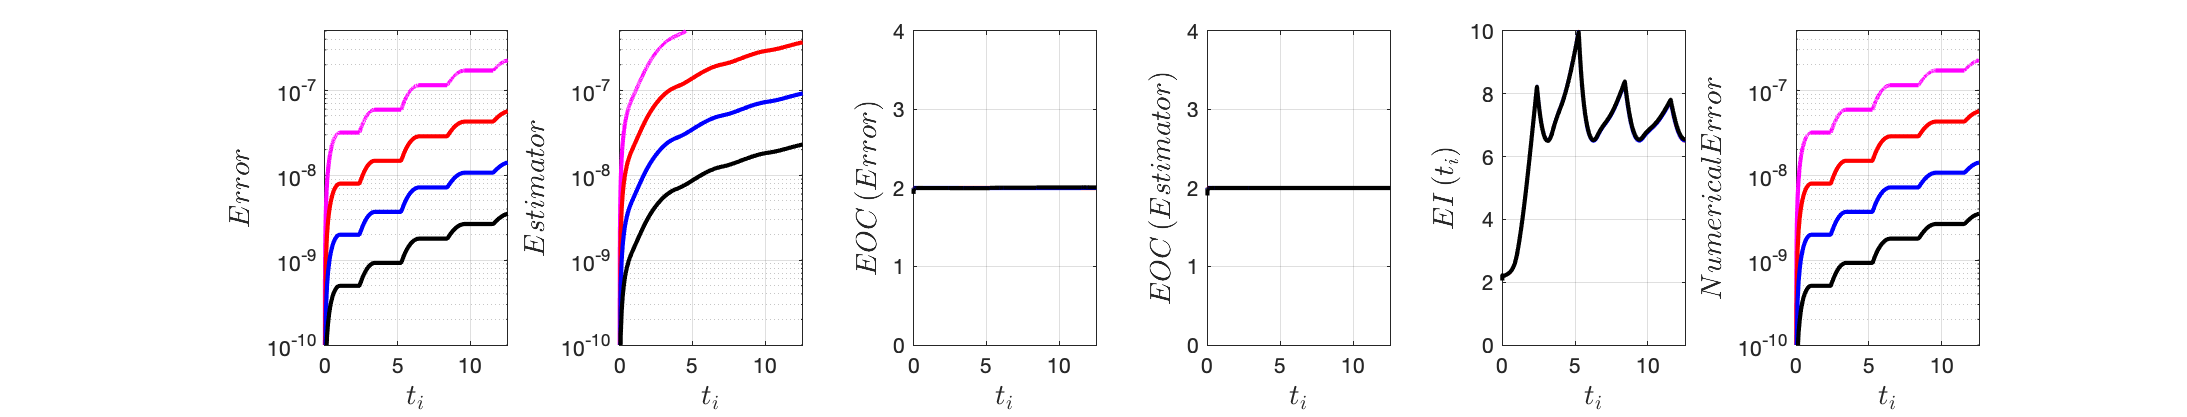
\includegraphics[scale=0.55]{fig_LeapFrogplots_1x5_sin_IC_harmonic_order_2_u5_v5_rec_george}	
	\caption{Reconstruction from Defn. \ref{defn_our_rec}. (from left to right) Error $e$ given by (\ref{eq_error_eR}), Estimator $\eta_1$ given by \ref{eq_bound_test},   EOC error, EOC Estimator, Effectivity Index.}
	\label{fig_all_in_one_our_rec_george_u5_v5}
\end{figure}
\begin{figure}[H]
	\hspace{-3cm}
	%\centering
	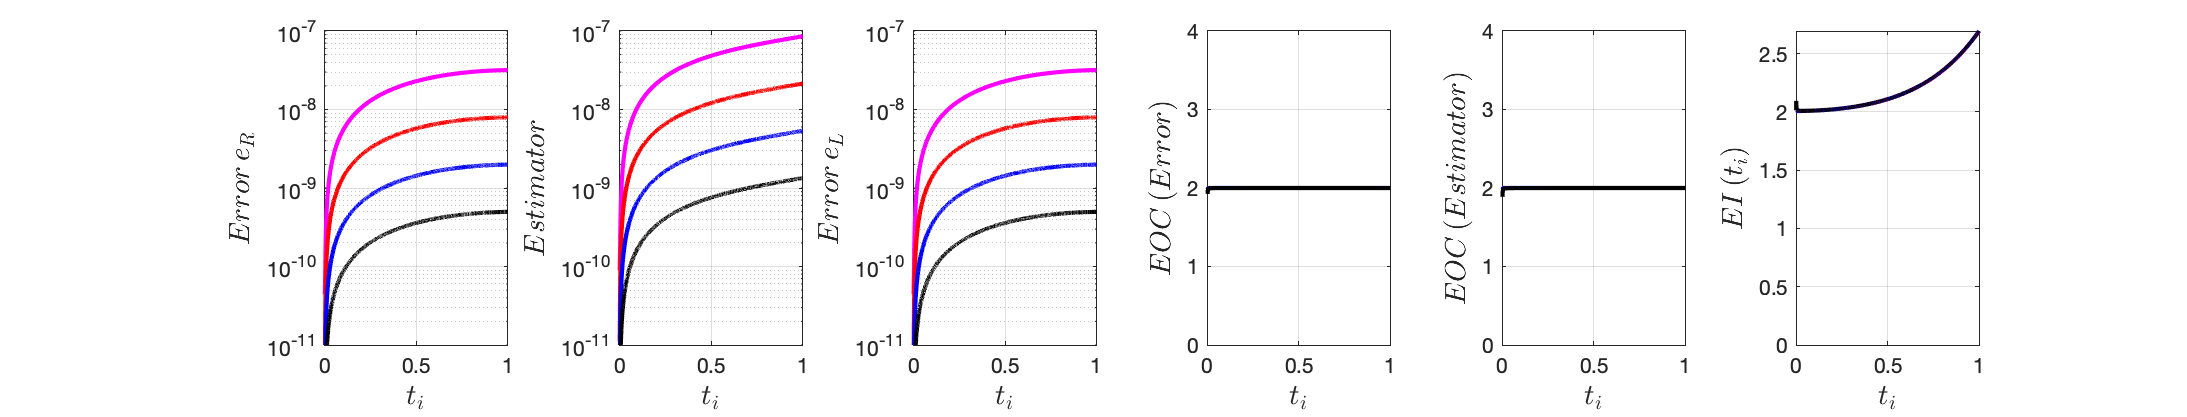
\includegraphics[scale=0.55]{fig_LeapFrogplots_1x5_sin_IC_harmonic_order_2_u5_v5_rec2}	
	\caption{Reconstruction from Defn. \ref{defn_our_rec2}. (from left to right) Error $e$ given by (\ref{eq_error_eR}), Estimator $\eta_1$ given by \ref{eq_bound_test},  EOC error, EOC Estimator, Effectivity Index.}
	\label{fig_all_in_one_our_rec_2_u5_v5}
\end{figure}
\begin{figure}[H]
	\hspace{-3cm}
	%\centering
	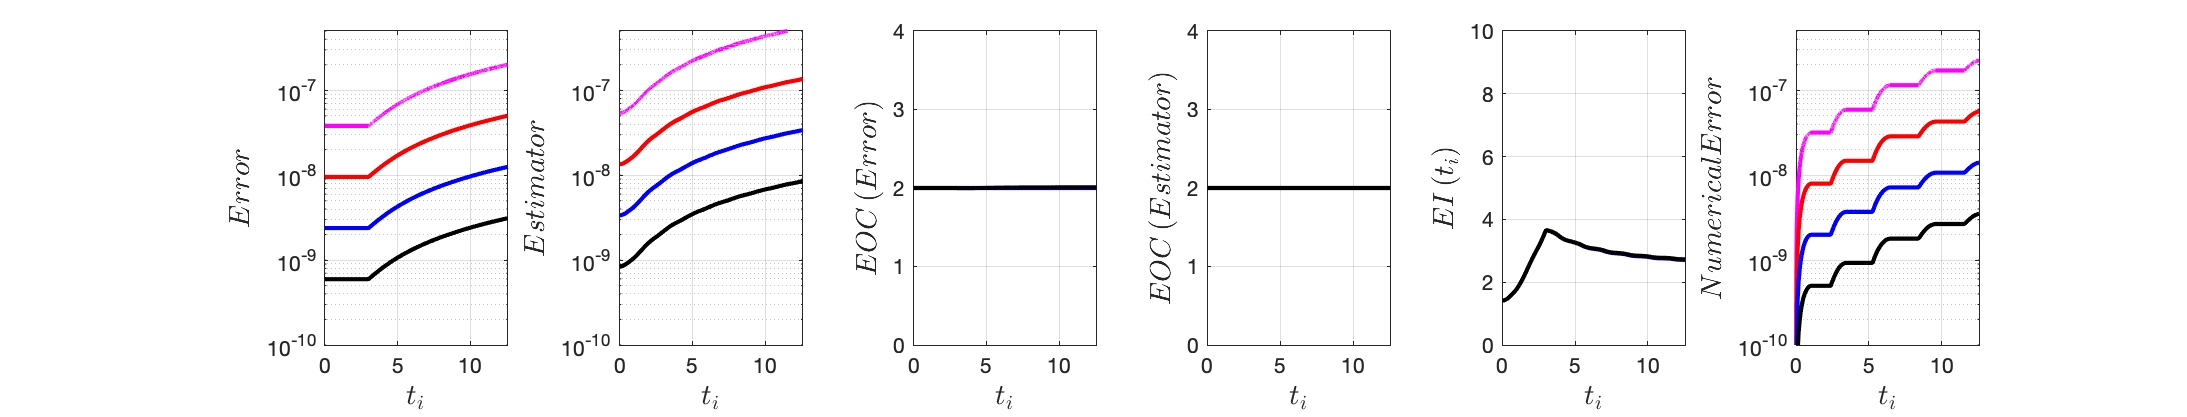
\includegraphics[scale=0.55]{fig_LeapFrogplots_1x5_sin_IC_harmonic_u5_v5_paperrec}	
	\caption{Paper rec. (from left to right) Error $e$ given by (\ref{eq_error_eR}), Estimator $\eta_1$ given by \ref{eq_bound_test},   EOC error, EOC Estimator, Effectivity Index.}
	\label{fig_all_in_one_paperrec_u05_v05}
\end{figure}
*/
\begin{figure}[H]
	\hspace{-3cm}
	%\centering
	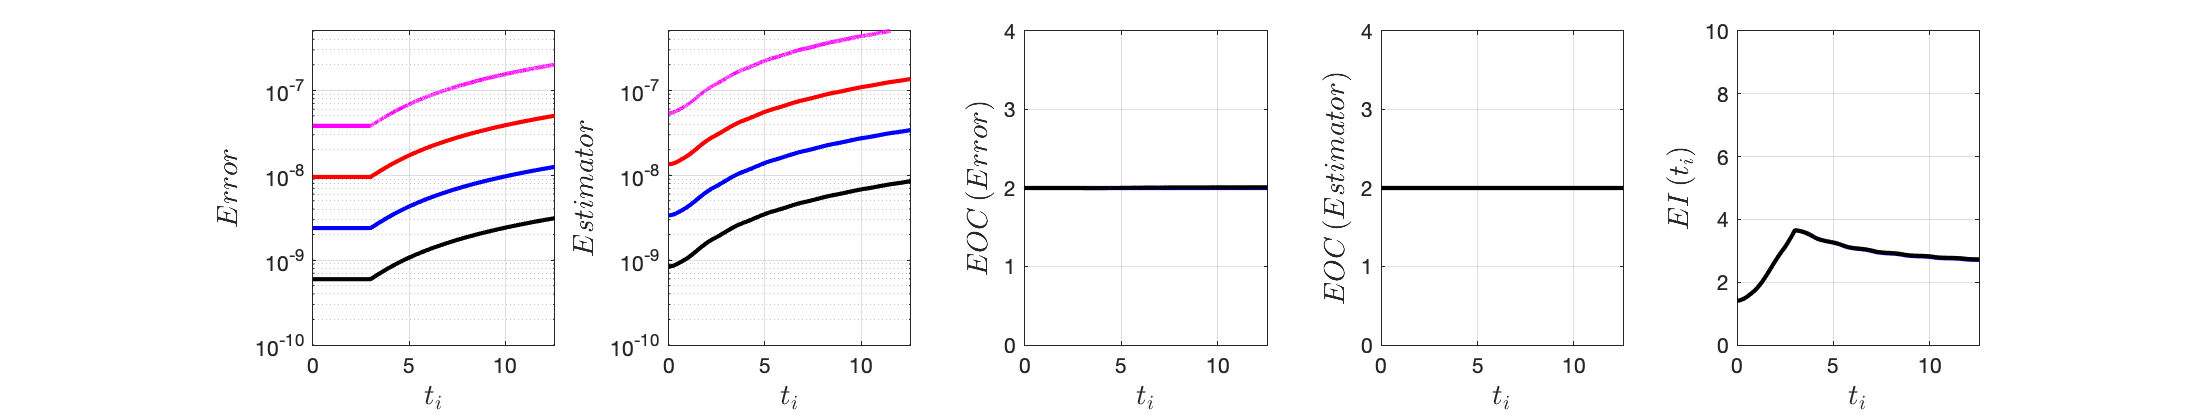
\includegraphics[scale=0.55]{fig_LeapFrogplots_1x5_sin_IC_harmonic_u5_v5_paperrec_poly_our_res}	
		\caption{Reconstruction from Defn. \ref{defn_rec_paper_poly}. (from left to right) Error $e$ given by (\ref{eq_error_eR}), Estimator $\eta_1$ given by (\ref{eq_bound_test}), EOC error, EOC Estimator, Effectivity Index.}
	\label{fig_all_in_one_paperrec_poly_u05_v05}
\end{figure}
\begin{figure}[H]
	\hspace{-3cm}
	%\centering
	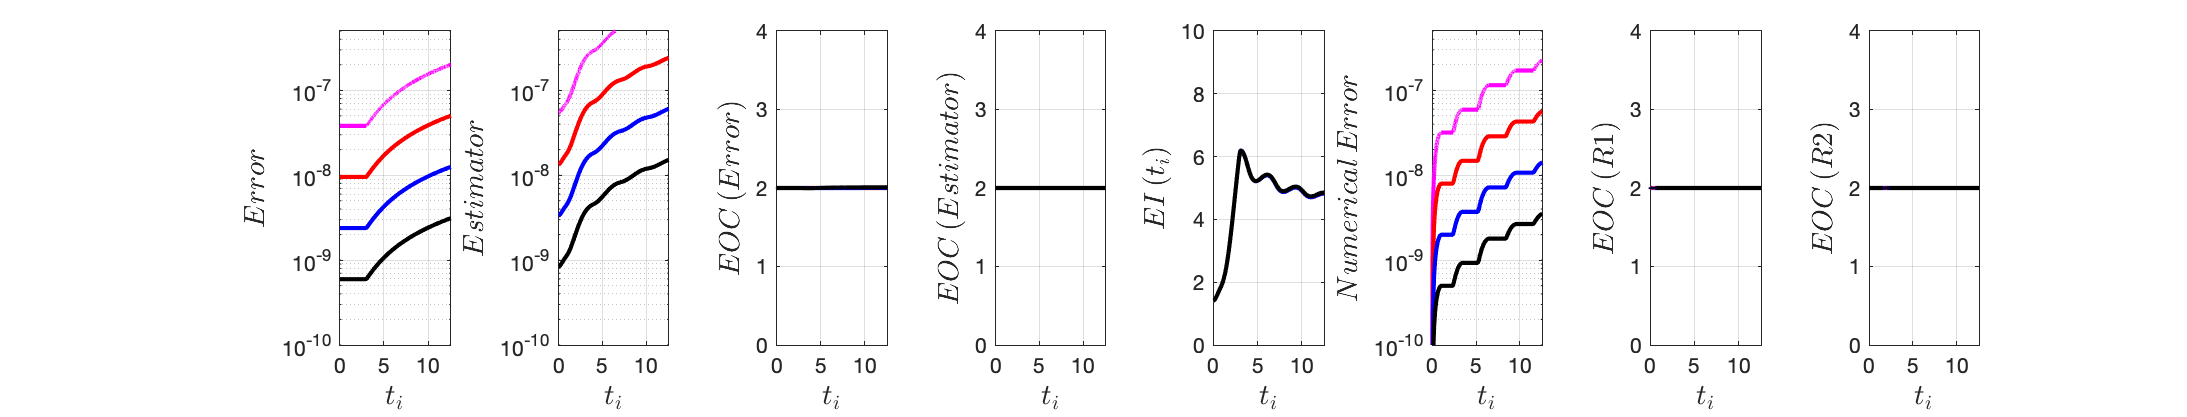
\includegraphics[scale=0.55]{fig_LeapFrogplots_1x5_sin_IC_harmonic_u5_v5_paperrec_poly_tristan}	
\caption{Reconstruction from Defn. \ref{defn_our_rec3} (from left to right) Error $e$ given by (\ref{eq_error_eR}), Estimator $\eta_1$ given by (\ref{eq_bound_test}), EOC error, EOC Estimator, Effectivity Index.}
	\label{fig_all_in_one_paperrec_poly_tristan_u5_v5}
\end{figure}

\subsection*{$u_0=0.6, v_0= 0.4$}
\/*
\begin{figure}[H]
	\hspace{-3cm}
	%\centering
	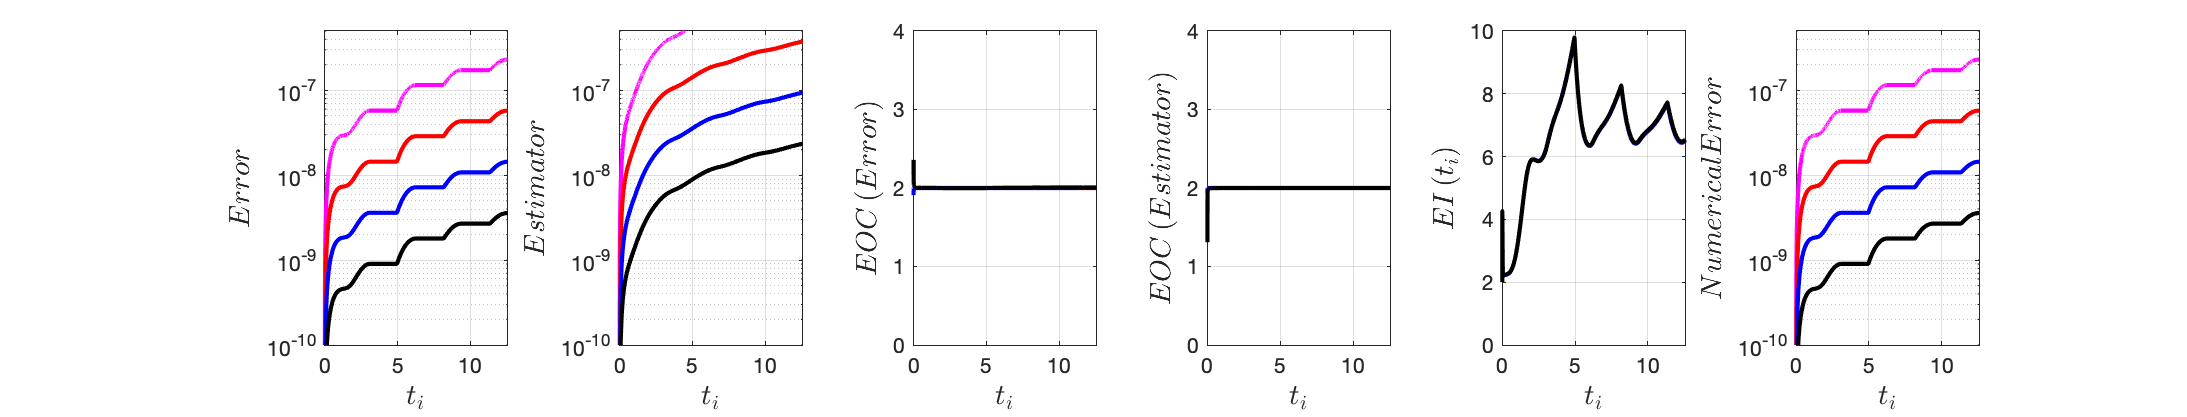
\includegraphics[scale=0.55]{fig_LeapFrogplots_1x5_sin_IC_harmonic_order_2_u6_v4_rec_george}	
	\caption{Reconstruction from Defn. \ref{defn_our_rec}. (from left to right) Error $e$ given by (\ref{eq_error_eR}), Estimator $\eta_1$ given by \ref{eq_bound_test}, EOC error, EOC Estimator, Effectivity Index.}
	\label{fig_all_in_one_our_rec_george_u6_v4}
\end{figure}
\begin{figure}[H]
	\hspace{-3cm}
	%\centering
	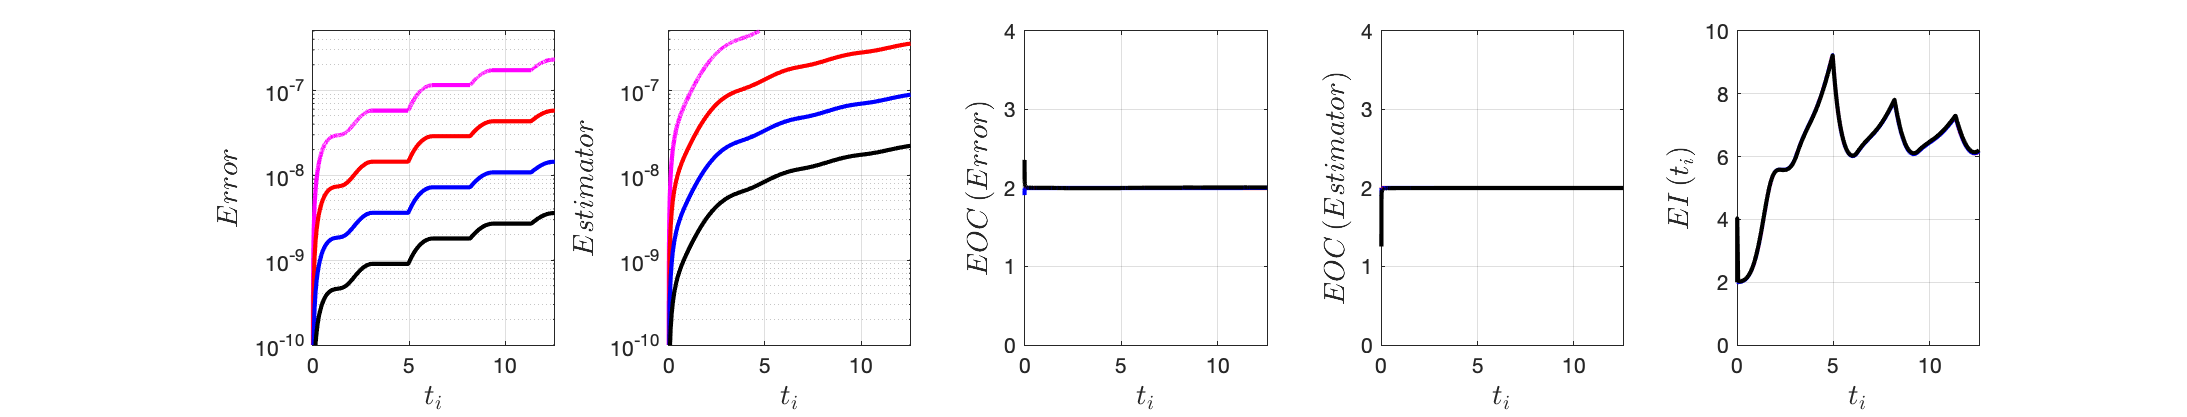
\includegraphics[scale=0.55]{fig_LeapFrogplots_1x5_sin_IC_harmonic_order_2_u6_v4_rec2}	
	\caption{Reconstruction from Defn. \ref{defn_our_rec2}. (from left to right) Error $e$ given by (\ref{eq_error_eR}), Estimator $\eta_1$ given by \ref{eq_bound_test},  EOC error, EOC Estimator, Effectivity Index.}
	\label{fig_all_in_one_our_rec_2_u6_v4}
\end{figure}
\begin{figure}[H]
	\hspace{-3cm}
	%\centering
	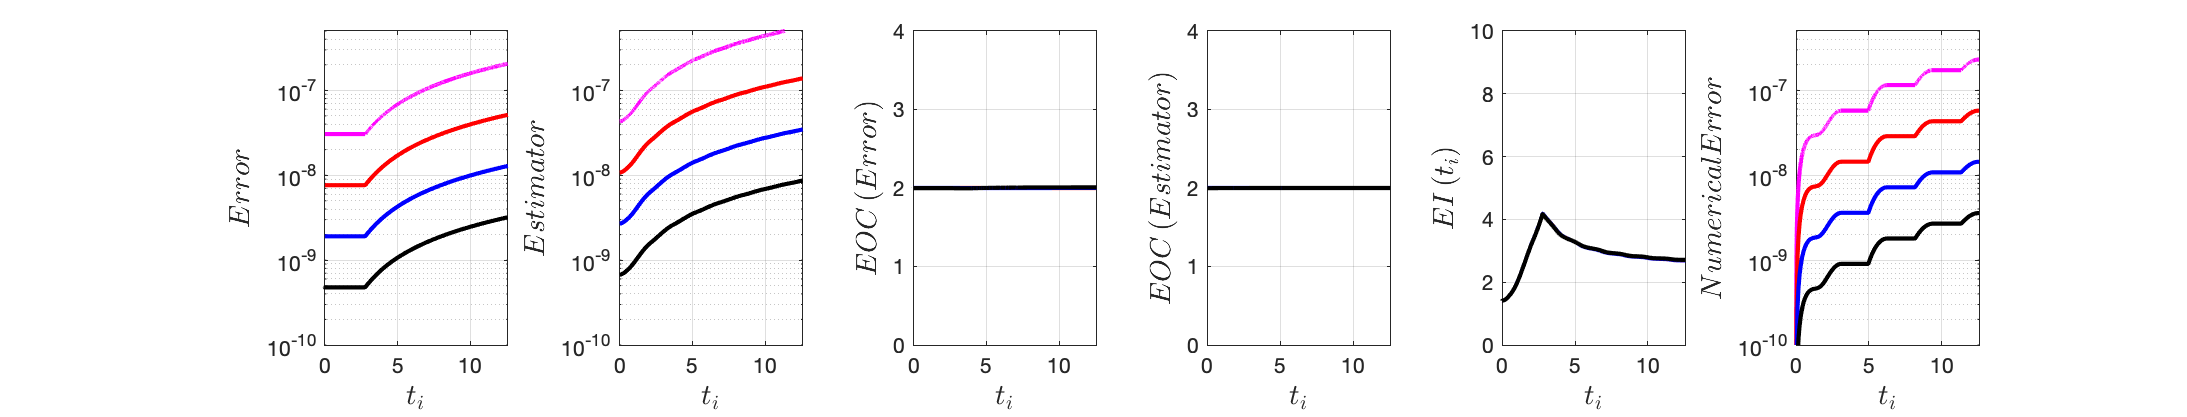
\includegraphics[scale=0.55]{fig_LeapFrogplots_1x5_sin_IC_harmonic_u6_v4_paperrec}	
	\caption{Paper rec. (from left to right) Error $e$ given by (\ref{eq_error_eR}), Estimator $\eta_1$ given by \ref{eq_bound_test},  EOC error, EOC Estimator, Effectivity Index.}
	\label{fig_all_in_one_paperrec_u06_v04}
\end{figure}
*/
\begin{figure}[H]
	\hspace{-3cm}
	%\centering
	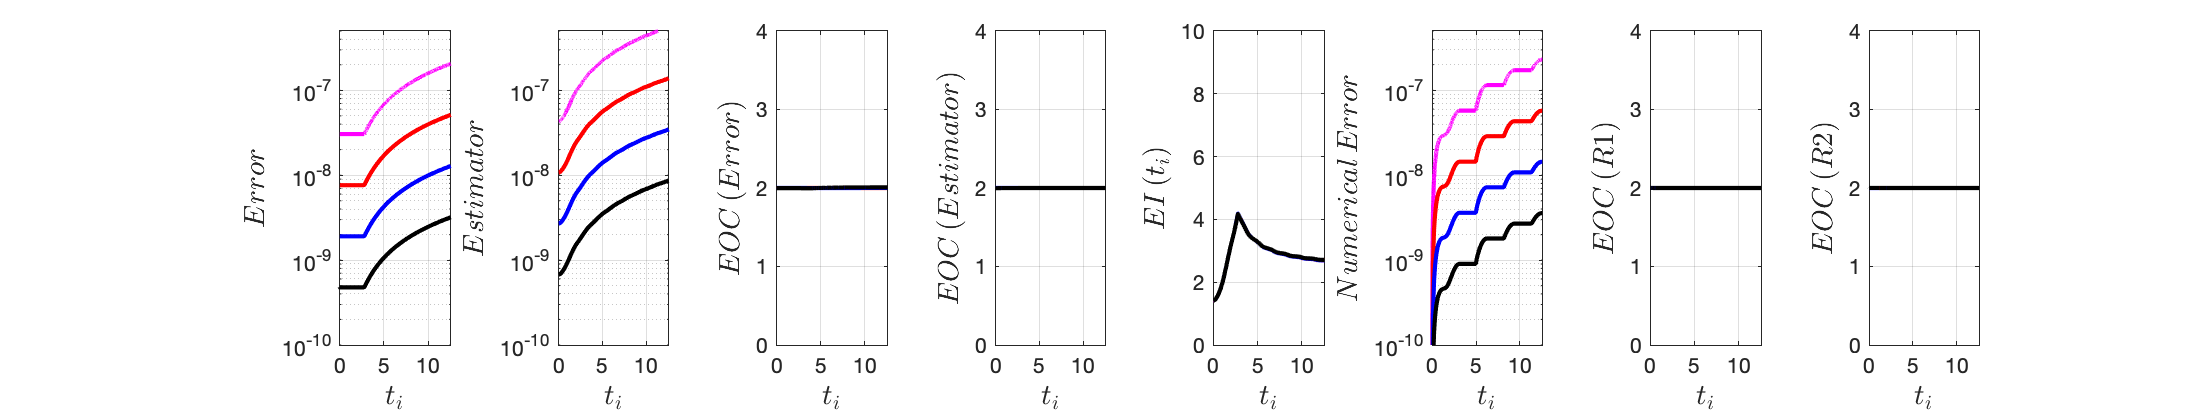
\includegraphics[scale=0.55]{fig_LeapFrogplots_1x5_sin_IC_harmonic_u6_v4_paperrec_poly_our_res}	
	\caption{Reconstruction from Defn. \ref{defn_rec_paper_poly}. (from left to right) Error $e$ given by (\ref{eq_error_eR}), Estimator $\eta_1$ given by (\ref{eq_bound_test}), EOC error, EOC Estimator, Effectivity Index.}
	\label{fig_all_in_one_paperrec_poly_u06_v04}
\end{figure}

\begin{figure}[H]
	\hspace{-3cm}
	%\centering
	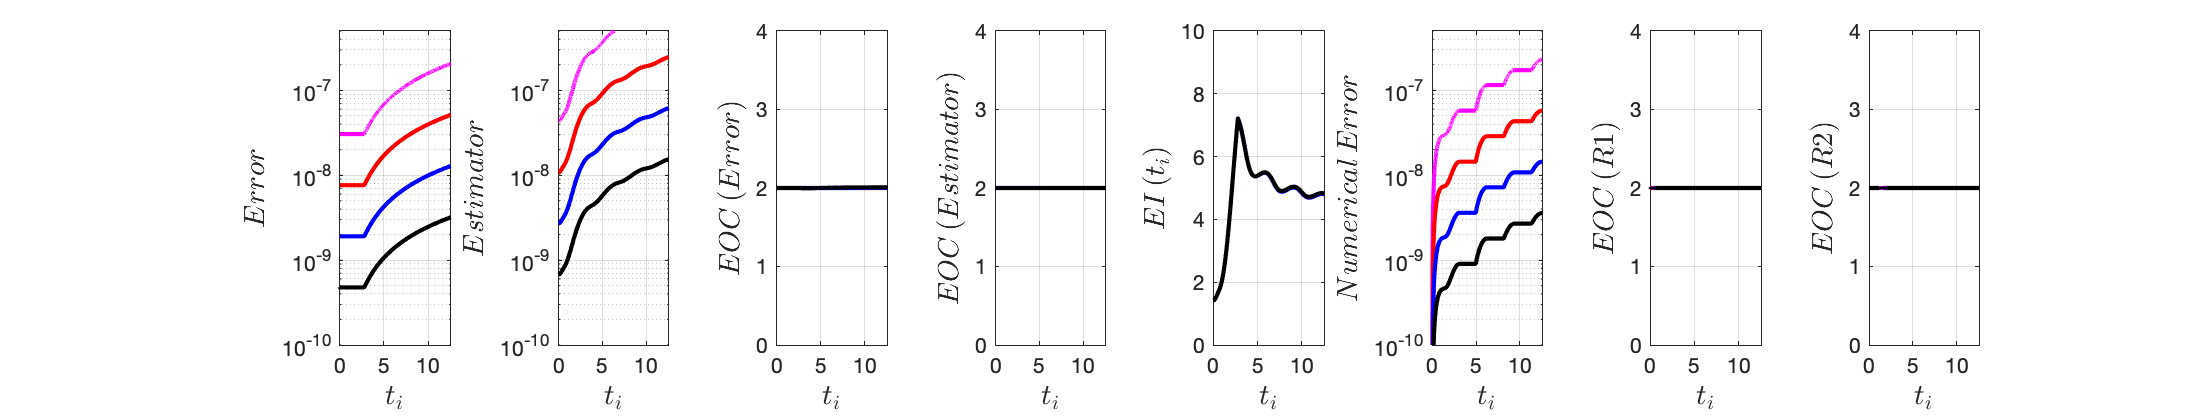
\includegraphics[scale=0.55]{fig_LeapFrogplots_1x5_sin_IC_harmonic_u6_v4_paperrec_poly_tristan}	
	\caption{Reconstruction from Defn. \ref{defn_our_rec3} (from left to right) Error $e$ given by (\ref{eq_error_eR}), Estimator $\eta_1$ given by (\ref{eq_bound_test}), EOC error, EOC Estimator, Effectivity Index.}
	\label{fig_all_in_one_paperrec_poly_tristan_u6_v4}
\end{figure}

\subsection*{$u_0=0.7, v_0= 0.3$}
\/*
\begin{figure}[H]
	\hspace{-3cm}
	%\centering
	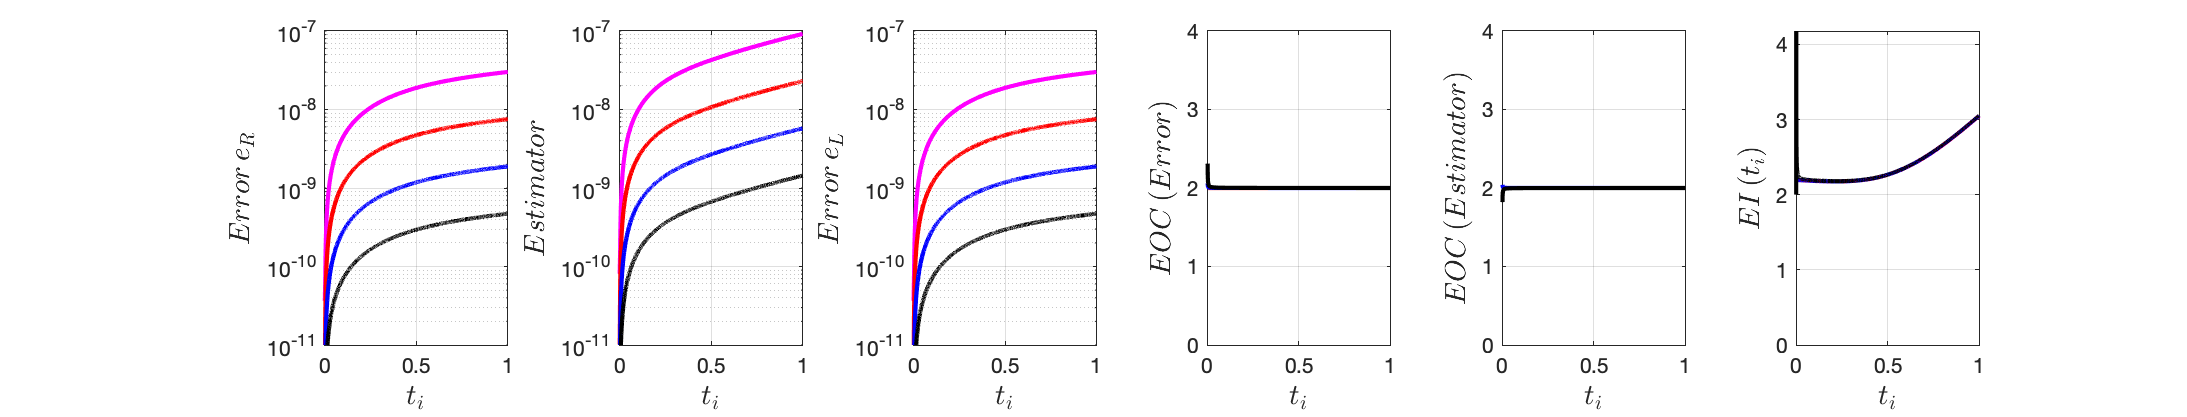
\includegraphics[scale=0.55]{fig_LeapFrogplots_1x5_sin_IC_harmonic_order_2_u7_v3_rec_george}	
	\caption{Reconstruction from Defn. \ref{defn_our_rec}. (from left to right) Error $e$ given by (\ref{eq_error_eR}), Estimator $\eta_1$ given by \ref{eq_bound_test},   EOC error, EOC Estimator, Effectivity Index.}
	\label{fig_all_in_one_our_rec_george_u7_v3}
\end{figure}
\begin{figure}[H]
	\hspace{-3cm}
	%\centering
	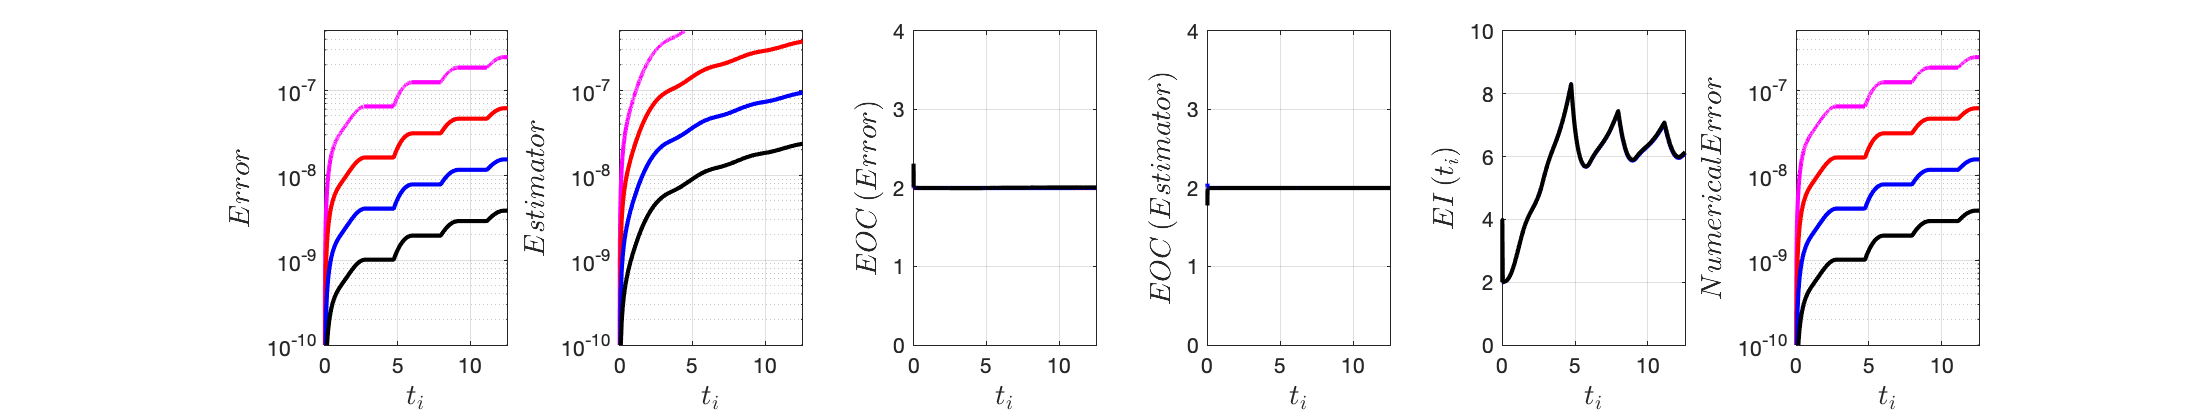
\includegraphics[scale=0.55]{fig_LeapFrogplots_1x5_sin_IC_harmonic_order_2_u7_v3_rec2}	
	\caption{Reconstruction from Defn. \ref{defn_our_rec2}. (from left to right) Error $e$ given by (\ref{eq_error_eR}), Estimator $\eta_1$ given by \ref{eq_bound_test},   EOC error, EOC Estimator, Effectivity Index.}
	\label{fig_all_in_one_our_rec_2_u7_v3}
\end{figure}
\begin{figure}[H]
	\hspace{-3cm}
	%\centering
	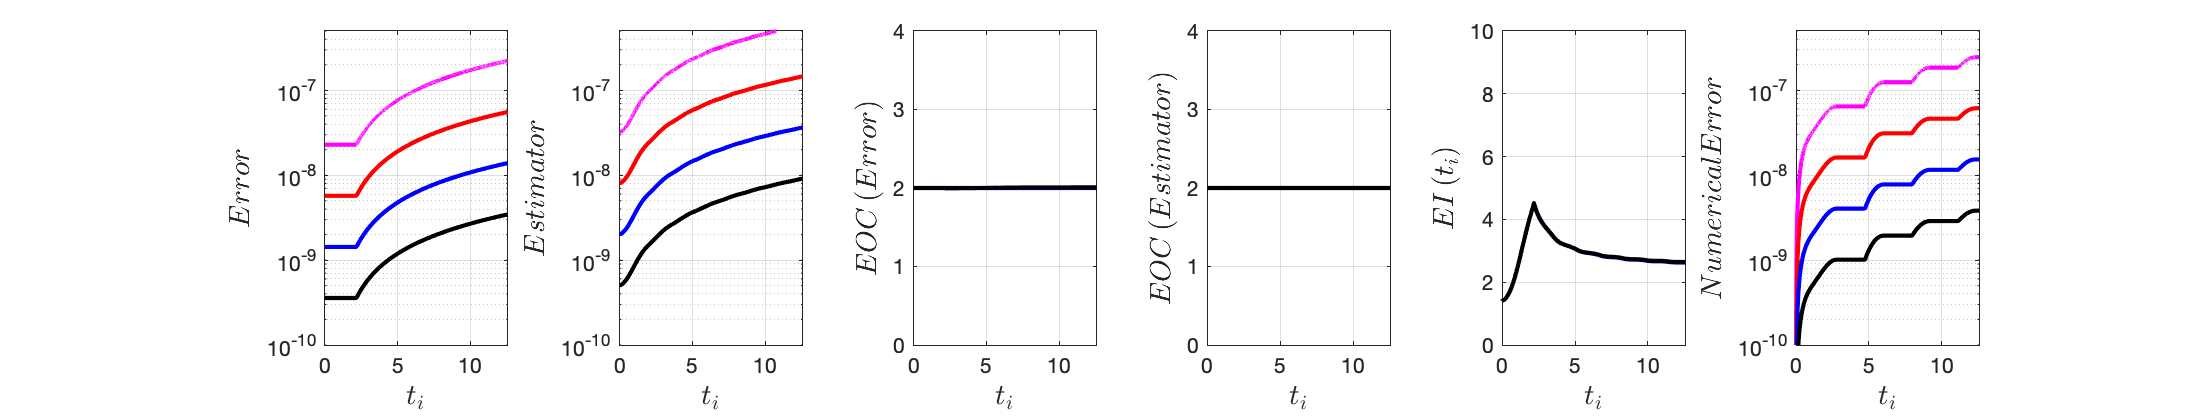
\includegraphics[scale=0.55]{fig_LeapFrogplots_1x5_sin_IC_harmonic_u7_v3_paperrec}	
	\caption{Paper rec. (from left to right) Error $e$ given by (\ref{eq_error_eR}), Estimator $\eta_1$ given by \ref{eq_bound_test},   EOC error, EOC Estimator, Effectivity Index.}
	\label{fig_all_in_one_paperrec_u07_v03}
\end{figure}
*/
\begin{figure}[H]
	\hspace{-3cm}
	%\centering
	\includegraphics[scale=0.55]{fig_LeapFrogplots_1x5_sin_IC_harmonic_u7_v3_paperrec_poly_our_res}	
	\caption{Reconstruction from Defn. \ref{defn_rec_paper_poly}. (from left to right) Error $e$ given by (\ref{eq_error_eR}), Estimator $\eta_1$ given by (\ref{eq_bound_test}), EOC error, EOC Estimator, Effectivity Index.}
	\label{fig_all_in_one_paperrec_poly_u07_v03}
\end{figure}

\begin{figure}[H]
	\hspace{-3cm}
	%\centering
	\includegraphics[scale=0.55]{fig_LeapFrogplots_1x5_sin_IC_harmonic_u7_v3_paperrec_poly_tristan}	
\caption{Reconstruction from Defn. \ref{defn_our_rec3} (from left to right) Error $e$ given by (\ref{eq_error_eR}), Estimator $\eta_1$ given by (\ref{eq_bound_test}), EOC error, EOC Estimator, Effectivity Index.}
	\label{fig_all_in_one_paperrec_poly_tristan_u7_v3}
\end{figure}

\subsection*{$u_0=0.8, v_0= 0.2$}
\/*
\begin{figure}[H]
	\hspace{-3cm}
	%\centering
	\includegraphics[scale=0.55]{fig_LeapFrogplots_1x5_sin_IC_harmonic_order_2_u8_v2_rec_george}	
	\caption{Reconstruction from Defn. \ref{defn_our_rec}. (from left to right) Error $e$ given by (\ref{eq_error_eR}), Estimator $\eta_1$ given by \ref{eq_bound_test},   EOC error, EOC Estimator, Effectivity Index.}
	\label{fig_all_in_one_our_rec_george_u8_v2}
\end{figure}
\begin{figure}[H]
	\hspace{-3cm}
	%\centering
	\includegraphics[scale=0.55]{fig_LeapFrogplots_1x5_sin_IC_harmonic_order_2_u8_v2_rec2}	
	\caption{Reconstruction from Defn. \ref{defn_our_rec2}. (from left to right) Error $e$ given by (\ref{eq_error_eR}), Estimator $\eta_1$ given by \ref{eq_bound_test},   EOC error, EOC Estimator, Effectivity Index.}
	\label{fig_all_in_one_our_rec_2_u8_v2}
\end{figure}
\begin{figure}[H]
	\hspace{-3cm}
	%\centering
	\includegraphics[scale=0.55]{fig_LeapFrogplots_1x5_sin_IC_harmonic_u8_v2_paperrec}	
	\caption{Paper rec. (from left to right) Error $e$ given by (\ref{eq_error_eR}), Estimator $\eta_1$ given by \ref{eq_bound_test},   EOC error, EOC Estimator, Effectivity Index.}
	\label{fig_all_in_one_paperrec_u08_v02}
\end{figure}
*/
\begin{figure}[H]
	\hspace{-3cm}
	%\centering
	\includegraphics[scale=0.55]{fig_LeapFrogplots_1x5_sin_IC_harmonic_u8_v2_paperrec_poly_our_res}	
	\caption{Reconstruction from Defn. \ref{defn_rec_paper_poly}. (from left to right) Error $e$ given by (\ref{eq_error_eR}), Estimator $\eta_1$ given by (\ref{eq_bound_test}), EOC error, EOC Estimator, Effectivity Index.}
	\label{fig_all_in_one_paperrec_poly_u08_v02}
\end{figure}
\begin{figure}[H]
	\hspace{-3cm}
	%\centering
	\includegraphics[scale=0.55]{fig_LeapFrogplots_1x5_sin_IC_harmonic_u8_v2_paperrec_poly_tristan}	
	\caption{Reconstruction from Defn. \ref{defn_our_rec3} (from left to right) Error $e$ given by (\ref{eq_error_eR}), Estimator $\eta_1$ given by (\ref{eq_bound_test}), EOC error, EOC Estimator, Effectivity Index.}
	\label{fig_all_in_one_paperrec_poly_tristan_u8_v2}
\end{figure}


\subsection*{$u_0=0.9, v_0= 0.1$}
\/*
\begin{figure}[H]
	\hspace{-3cm}
	%\centering
	\includegraphics[scale=0.55]{fig_LeapFrogplots_1x5_sin_IC_harmonic_order_2_u9_v1_rec_george}	
	\caption{Reconstruction from Defn. \ref{defn_our_rec}. (from left to right) Error $e$ given by (\ref{eq_error_eR}), Estimator $\eta_1$ given by \ref{eq_bound_test},  EOC error, EOC Estimator, Effectivity Index.}
	\label{fig_all_in_one_our_rec_george_u9_v1}
\end{figure}
\begin{figure}[H]
	\hspace{-3cm}
	%\centering
	\includegraphics[scale=0.55]{fig_LeapFrogplots_1x5_sin_IC_harmonic_order_2_u9_v1_rec2}	
	\caption{Reconstruction from Defn. \ref{defn_our_rec2}. (from left to right) Error $e$ given by (\ref{eq_error_eR}), Estimator $\eta_1$ given by \ref{eq_bound_test},  EOC error, EOC Estimator, Effectivity Index.}
	\label{fig_all_in_one_our_rec_2_u9_v1}
\end{figure}
\begin{figure}[H]
	\hspace{-3cm}
	%\centering
	\includegraphics[scale=0.55]{fig_LeapFrogplots_1x5_sin_IC_harmonic_u9_v1_paperrec}	
	\caption{Paper rec. (from left to right) Error $e$ given by (\ref{eq_error_eR}), Estimator $\eta_1$ given by \ref{eq_bound_test},   EOC error, EOC Estimator, Effectivity Index.}
	\label{fig_all_in_one_paperrec_u09_v01}
\end{figure}
*/
\begin{figure}[H]
	\hspace{-3cm}
	%\centering
	\includegraphics[scale=0.55]{fig_LeapFrogplots_1x5_sin_IC_harmonic_u9_v1_paperrec_poly_our_res}	
	\caption{Reconstruction from Defn. \ref{defn_rec_paper_poly}. (from left to right) Error $e$ given by (\ref{eq_error_eR}), Estimator $\eta_1$ given by (\ref{eq_bound_test}), EOC error, EOC Estimator, Effectivity Index.}
	\label{fig_all_in_one_paperrec_poly_u09_v01}
\end{figure}
\begin{figure}[H]
	\hspace{-3cm}
	%\centering
	\includegraphics[scale=0.55]{fig_LeapFrogplots_1x5_sin_IC_harmonic_u9_v1_paperrec_poly_tristan}	
\caption{Reconstruction from Defn. \ref{defn_our_rec3} (from left to right) Error $e$ given by (\ref{eq_error_eR}), Estimator $\eta_1$ given by (\ref{eq_bound_test}), EOC error, EOC Estimator, Effectivity Index.}
	\label{fig_all_in_one_paperrec_poly_tristan_u9_v1}
\end{figure}


\subsection*{$u_0=1.0, v_0= 0$}
\/*
\begin{figure}[H]
	\hspace{-3cm}
	%\centering
	\includegraphics[scale=0.55]{fig_LeapFrogplots_1x5_sin_IC_harmonic_order_2_u10_v0_rec_george}	
	\caption{Reconstruction from Defn. \ref{defn_our_rec}. (from left to right) Error $e$ given by (\ref{eq_error_eR}), Estimator $\eta_1$ given by \ref{eq_bound_test},  EOC error, EOC Estimator, Effectivity Index.}
	\label{fig_all_in_one_our_rec_george_u10_v0}
\end{figure}
\begin{figure}[H]
	\hspace{-3cm}
	%\centering
	\includegraphics[scale=0.55]{fig_LeapFrogplots_1x5_sin_IC_harmonic_order_2_u10_v0_rec2}	
	\caption{Reconstruction from Defn. \ref{defn_our_rec2}. (from left to right) Error $e$ given by (\ref{eq_error_eR}), Estimator $\eta_1$ given by \ref{eq_bound_test},   EOC error, EOC Estimator, Effectivity Index.}
	\label{fig_all_in_one_our_rec_2_u10_v0}
\end{figure}
\begin{figure}[H]
	\hspace{-3cm}
	%\centering
	\includegraphics[scale=0.55]{fig_LeapFrogplots_1x5_sin_IC_harmonic_u10_v0_paperrec}	
	\caption{Paper rec. (from left to right) Error $e$ given by (\ref{eq_error_eR}), Estimator $\eta_1$ given by \ref{eq_bound_test}, EOC error, EOC Estimator, Effectivity Index.}
	\label{fig_all_in_one_paperrec_u10_v1}
\end{figure}
*/
\begin{figure}[H]
	\hspace{-3cm}
	%\centering
	\includegraphics[scale=0.55]{fig_LeapFrogplots_1x5_sin_IC_harmonic_u10_v0_paperrec_poly_our_res}	
	\caption{Reconstruction from Defn. \ref{defn_rec_paper_poly}. (from left to right) Error $e$ given by (\ref{eq_error_eR}), Estimator $\eta_1$ given by (\ref{eq_bound_test}), EOC error, EOC Estimator, Effectivity Index.}
	\label{fig_all_in_one_paperrec_poly_u10_v1}
\end{figure}

\begin{figure}[H]
	\hspace{-3cm}
	%\centering
	\includegraphics[scale=0.55]{fig_LeapFrogplots_1x5_sin_IC_harmonic_u10_v0_paperrec_poly_tristan}	
\caption{Reconstruction from Defn. \ref{defn_our_rec3} (from left to right) Error $e$ given by (\ref{eq_error_eR}), Estimator $\eta_1$ given by (\ref{eq_bound_test}), EOC error, EOC Estimator, Effectivity Index.}
	\label{fig_all_in_one_paperrec_poly_tristan_u10_v0}
\end{figure}



\section{Discussion}\label{sec:discussion}
In this section we discuss the findings from the numerical experiments.  Briefly, we tested the aposterior bound (\ref{eq_bound_test}) with two different reconstructions: \ref{defn_rec_paper_poly} from \cite{georgoulis2016posteriori} and the reconstruction form Defn. \ref{defn_our_rec3} . The error was measured in the $L^{\infty}-$norm in time. 

 We investigated the temporal evolution of the error (\ref{eq_error_eR})  and the bound (\ref{eq_bound_test}) and we compared the performances of the  reconstructions in terms of their EOCs and the effectivity index.

Firstly,  both reconstructions are of optimal order in all numerical experiments in \S \ref{sec:num_exp}. This means that they both converged with the same order as the underlying error of the numerical scheme.  
Additionally, they both lead to robust a posteriori estimates, in the sense that the estimate does not become infinite while the error is finite.

The difference between them reconstructions is in terms of their efficiency.  The reconstruction in (\ref{eq_rec_paper}) led to a sharper estimate for the bound (\ref{eq_bound_test}) compared to the reconstructions from Defn.  \ref{defn_our_rec3}.  This can be seen from the Effectivity Index (last subplot on the right) in the figures in \S\ref{sec:num_exp}.  Notice that the lead contribution to the bound comes from $\mathcal{R}_2$ which is the right-most plot in each figure.

This difference in efficiency between the two reconstructions can be understood by substituting the exact solution in the coefficients.  It is enough to look at $\mathcal{R}_2$ because it is the lead contribution in both cases.  We start  from (\ref{defn_rec_paper_poly}).  We have that 
\begin{equation}
\mathcal{R}_2 = \rec{U}'\qp{t}- \rec{V}\qp{t},
\end{equation}
Starting from Defn. \ref{defn_rec_paper_poly}, looking at the interval $t\in\qb{t^{n}, t^{n+1/2}}$, we have that
\begin{equation*}
\begin{aligned}
\rec{V}\qp{t}=	& V^{n-1/2}
+\qp{\frac{1}{4}U^{n+1}-U^n-\frac{1}{4}U^{n-1}}\qp{t-t^{n-1/2}}
-\frac{1}{4\Delta t}\qp{U^{n+1}-U^{n-1}}\qp{t-t^{n-1/2}}^2
\end{aligned}
\end{equation*}
and 
\begin{equation*}
\begin{aligned}
\rec{U}'\qp{t}=	-\frac{1}{4}V^{n+3/2}+V^{n+1/2}+\frac{1}{4}V^{n-1/2}
+\frac{1}{2\Delta t}\qp{V^{n+3/2}-V^{n-1/2}}\qp{t-t^{n}}.
\end{aligned}
\end{equation*}
In this case, we are interested in the constants in these expressions, as they will lead to the leading order error term:
\begin{equation*}
\rec{U}'-\rec{V} = -\frac{1}{4}\qp{V^{n+3/2}-V^{n+1/2}+3V^{n-1/2}} + h.o.t.
\end{equation*}.

Substituting the exact solutions $u$ and $v$ for $U$ and $V$ and expanding up to order 2 we obtain the  leading order error term 
\begin{equation}
\qp{\frac{1}{2}v'\qp{t}-\frac{1}{4}v''\qp{t}}\Delta t.
\end{equation}

In the case of the reconstruction from Defn. \ref{defn_our_rec3}, we obtain
\begin{equation*}
\begin{aligned}
\rec{U}'-\rec{V} &=\frac{1}{\Delta t}\qp{U^{n+1}-U^n+\frac{1}{2}\Delta t^2 U^n} -V^{n-1/2}+ h.o.t.,\\
&= V^{n+1/2}-V^{n-1/2}+\frac{\Delta t}{2}U^n.
\end{aligned}
\end{equation*}.
Substituting in the exact solutions yields the relevant error term as 
\begin{equation}
\qp{v'\qp{t}+\frac{1}{2} u\qp{t}}\Delta t=\qp{v'\qp{t}-\frac{1}{2} u''\qp{t}}\Delta t=\qp{v'\qp{t}-\frac{1}{2} v'\qp{t}}\Delta t
\end{equation}
In both cases, the lead contribution to the bound (\ref{eq_bound_test}) comes from $\mathcal{R}_2$ in (\ref{eq_residuals_our}), which is $\mathcal{O}\qp{\Delta t^2}$ in the bound.  However, in the case of (\ref{eq_rec_paper_poly_alternative}) the constant in front of this term is smaller compared to that in Defn. \ref{defn_our_rec3}.  This can be confirmed by visually inspecting the last two plots on the right for any of the Figures in \S \ref{sec:num_exp}, which illustrate the evolution of $\mathcal{R}_1$ and $\mathcal{R}_2$.  

\section{Conclusion}
In this chapter we tested the reconstruction of \cite{georgoulis2016posteriori} against one derived using our framework in the context of a model problem given by (\ref{eq_model_problem}), discretized by a reformulated leap-frog scheme. We have found that both reconstructions lead to reliable, robust a posteriori estimates.  The difference between them is in terms of efficiency.  The reconstruciton from \cite{georgoulis2016posteriori} leads to a sharper bound compared to that presented in Defn. \ref{defn_our_rec3}, on account of the smaller constant in the leading order error term. 

\bibliography{apostfd_bibdesk}
\bibliographystyle{ieeetr}
\end{document}